%%%%%%%%%%%%%%%%%%%%%%%%%%%%%%%%%%%%%%%%%%%%%%%%%%%%%%%%%%%%%%%%%%%%%%
% Lớp 11 | Đường thẳng, mặt phẳng. Quan hệ song song trong | Hai đường thẳng song song
% Dạng 1H4?2-4: Tìm giao điểm của đường thẳng và mặt phẳng
% Số câu: 49  (sinh tự động bởi tach_cau.py; từ nay thầy sửa trực tiếp file này)
%%%%%%%%%%%%%%%%%%%%%%%%%%%%%%%%%%%%%%%%%%%%%%%%%%%%%%%%%%%%%%%%%%%%%%

%%%%%%%%%%%%%%%% TRẮC NGHIỆM 4 PHƯƠNG ÁN %%%%%%%%%%%%%%%%

% nguồn: Ok_Toan11_TracNghiem_Lan2
\begin{ex}%[1H4N2-4]%[ma:0e069577]
	Cho lăng trụ $ABCD.A'B'C'D'$ có hai đáy là các hình bình hành. Các điểm $M$, $N$, $P$ lần lượt là trung điểm của cạnh $AD$, $BC$, $CC'$ (tham khảo hình vẽ). Xét các khẳng  định sau:
	\begin{center}
		\begin{tikzpicture}[scale=0.8,font=\footnotesize,line join=round,line cap=round,>=stealth]
				 \coordinate (A) at (0,0);
				\coordinate (B) at (-2,-2); 
				\coordinate (D) at (6,0); 
				\coordinate (C)  at ($(B)+(D)-(A)$);
				\foreach \i  in {A,B,C,D}{\coordinate (\i') at ($(\i)+(0,5)$);}
				\coordinate (M) at ($(A)!0.5!(D)$); 
				\coordinate (N)  at ($(B)!0.5!(C)$);
				\coordinate  (P) at ($(C')!0.5!(C)$);
				\draw  (B)--(C)--(D);
				\draw  (B)--(B')
					(C)--(C') 
					 (D)--(D')
					 (A')--(D')--(C')--(B')--(A')
					(N)--(P); 
				 \draw[dashed,thin] (A')--(A)--(B)
					 (A)--(D)
					 (P)--(M)--(N);
				\foreach \i/\g in {A'/170,B'/170,C'/-10,D'/0,A/30,B/140,C/-20,D/10,M/150,N/120,P/10}{\draw[fill=blue](\i) circle  (1pt)
					 ($(\i)+(\g:5mm)$) node[scale=1]{$\i$};}
			\end{tikzpicture}
	\end{center}
	\begin{enumerate}
		\item Mặt phẳng $\left(MNP\right)$ cắt  cạnh $A'D'$.
		\item Mặt phẳng $\left(MNP\right)$ cắt cạnh $DD'$  tại trung điểm của $DD'$.
		\item Mặt  phẳng $\left(MNP\right)$ song song với mặt phẳng $\left(ABC'D'\right)$.
	\end{enumerate}
	Trong các khẳng  định trên, số khẳng định đúng là
	\choice 
		 {$4$}
		 {$3$}
		{\True$2$} 
		 {$1$}
	 \loigiai{
		\begin{itemize}
			\item Lấy $E$ là trung điểm $D D^{\prime} \Rightarrow E P \parallel C D \parallel  M N$ suy ra $(MNP)\equiv (MNPE)$.
			Do đó $(MNP)\cap  DD^{\prime}=E$ với $E$ là trung điểm $D D^{\prime}$ nên b) đúng.
			\item Trong $\left(ADD^{\prime}A^{\prime}\right)$ có $ME$ cắt tia $A^{\prime}D^{\prime}$ tại $F$ suy ra $(MNPE)\cap  A^{\prime}D^{\prime}=\{F\}$.
			Ta có $AMFD^{\prime}$ là hình  bình hành (do $MF \parallel AD^{\prime};\; AM \parallel D^{\prime}F$) nên
			 \[
			AM  = D^{\prime}F = \dfrac{1}{2}A^{\prime}D^{\prime} \;\Rightarrow\; A^{\prime}F = \dfrac{3}{2}A^{\prime}D.
			 \]
			Nên $F$  không thuộc cạnh $A^{\prime}D^{\prime}$, do đó a) sai.
			\item Ta có $ME  \parallel AD^{\prime}$ (do $ME$ là đường trung bình của $\triangle DAD^{\prime}$) và $MN \parallel AB$ nên $(MNP)\parallel (ABC^{\prime}D^{\prime})$, do đó c) đúng.
		\end{itemize}
	} 
\end{ex}

% nguồn: Ok_Toan11_TracNghiem_Lan2
\begin{ex}%[1H4H2-4]%[ma:91b811f8]
	Cho bốn điểm $A$, $B$, $C$, $D$ không đồng phẳng. Gọi $M$, $N$ lần lượt là trung điểm của $AC$ và $BC$. Trên đoạn $BD$ lấy điểm $P$ sao cho $BP=2PD$. Giao điểm của đường thẳng $CD$  và mặt phẳng $(MNP)$ là giao điểm của cặp đường thẳng nào sau đây?
	 \choice
		{\True $CD$  và $NP$}
		{$CD$ và  $MN$}
		{$CD$  và $MP$}
		{$CD$ và  $AP$}
	\loigiai{ 
	\immini{Ta  có \[\heva{&N\in BC\\&P\in BD} \Rightarrow NP\subset(BCD).\]
		 Suy ra $NP$, $CD$ đồng phẳng.\\
		Gọi $E$ là giao điểm của $NP$  và $CD$.\\
		Mà $NP\subset(MNP)$ nên $CD\cap(MNP)=E$.} 
		{\begin{tikzpicture}[scale=1,font=\footnotesize,line join=round,line cap=round,>=stealth]
		\coordinate (B) at (0,0); 
		\coordinate (D)  at (3,0);
		\coordinate (C) at  (1.5,-3);
		\coordinate (A) at  (0,3.3);
		\coordinate  (M) at ($(C)!0.5!(A)$);
		\coordinate  (N) at ($(C)!0.5!(B)$);
		 \coordinate (P) at ($(B)!0.8!(D)$);
		\coordinate (E) at (intersection cs: first line={(N)--(P)},second  line={(C)--(D)});
		\draw (B)  -- (C)
			(C) -- (D) 
			(A) -- (B) 
			(A) --  (C)
			(A) -- (D) 
			(C) -- (M) 
			(C) -- (N) 
			(C) -- (D) 
			(E) -- (D) 
			(E) -- (M); 
		\draw[dashed] (D) --  (B)
			(N) --  (P)
			(E)  -- (P);
		\filldraw (E) circle (1pt)  node[font=\small,above] {E};
		\foreach \pt/\pos in {A/above,B/below left,C/below right,D/below right,M/above left,N/left,P/above} 
		\filldraw (\pt) circle (1pt) node[font=\small,\pos]  {\pt};
	\end{tikzpicture}
		 }
	 }
\end{ex}

% nguồn: Ok_Toan11_TracNghiem_Lan2
\begin{ex}%[1H4H2-4]%[ma:6f1691f9]
	Cho tứ diện $ABCD$ có $M$, $N$ theo thứ tự là trung điểm của $AB$, $BC$. Gọi $P$ là điểm thuộc cạnh $CD$ sao cho $CP=2PD$ và $Q$ là điểm thuộc cạnh $AD$ sao cho bốn điểm $N$, $P$, $Q$ đồng phẳng. Khẳng định nào sau  đây đúng?
	\choice 
		{$Q$ là trung điểm của đoạn thẳng  $AC$}
		 {$DQ=2AQ$}
		{\True $AQ=2DQ$} 
		 {$AQ=3DQ$}
	 \loigiai{
		\begin{center}
			\begin{tikzpicture}[scale=1,font=\footnotesize,line join=round,line cap=round,>=stealth]
					\path 
						(0,0) coordinate (B) 
						(3,-2) coordinate (C) 
						 (4,0) coordinate (D)
						(1.2,3.4)  coordinate (A)
						($(A)!0.5!(B)$) coordinate (M) 
						($(B)!.5!(C)$) coordinate (N) 
						($(C)!2/3!(D)$) coordinate (P) 
						($(A)!2/3!(D)$) coordinate  (Q);
					\draw (D)--(A)--(B)--(C)--cycle  (A)--(C)
						 (M)--(N)
						(P)--(Q); 
					\draw[dashed]  (B)--(D)
						 (N)--(P)
						 (M)--(Q);
					\foreach \p/\q  in {A/90,B/180,C/-90,D/40,M/140,N/230,P/0,Q/0}
					\fill (\p) circle (1.0pt) 
						($(\p)+(\q:2.5mm)$)  node{$\p$};
				\end{tikzpicture}
		\end{center}
		Xét  $\triangle ABC$ có $MN$ là đường trung bình nên $MN\parallel AC$.\\
		Ta có $\heva{&P\in (MNP)\cap (ACD)\\&MN\subset (MNP)\\&AC\subset (ACD).}$\\ 
		Suy ra, $(MNP)\cap (ACD)=d$  với $d$ đi qua $P$ và song song với $AC$; cắt $AD$ tại $Q$.\\
		Mặt khác, trong $\triangle ACD$ có $\heva{&CP=2PD\\&PQ\parallel AC}$ nên  $AQ=2DQ$.
	} 
\end{ex}

% nguồn: Ok_TracNghiemLop11_Lan1
\begin{ex}%[1H4H2-4]%[ma:c3271fb8]
	
	Cho tứ diện $ ABCD$. Gọi $ M$ và $ N$ lần lượt là trung điểm của $ BC$ và $ AD$;  $ G$ là trung điểm của $ MN$. Trong các khẳng định sau, khẳng định nào {\bf sai}?
	\choice 
		{$ BG\cap\left(ACD\right)=B'\,\,;\,\,B'$ là  trọng tâm tam giác $ ACD$}
		{$  G$ là trọng tâm tứ diện $ ABCD$}
		{$ AG\cap\left(BCD\right)=A'\,\,;\,\,A'$ là trọng tâm tam giác $ BCD$} 
		{\True $ G$ là trọng tâm tam giác  $ ADM$}
	 \loigiai{
		\begin{center}
			\tikzset{every picture/.style={line width=0.75pt}} 
			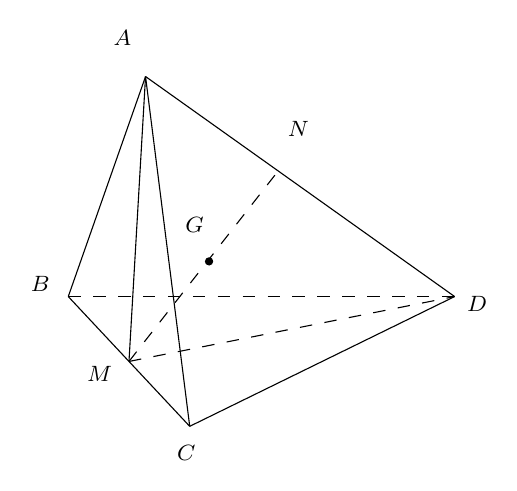
\begin{tikzpicture}[x=0.75pt,y=0.75pt,yscale=-1,xscale=1]
					\draw [dash  pattern={on 4.5pt off 4.5pt}] (231.6,157.55) -- (417.75,157.55);
					\draw (231.6,157.55)  -- (290.11,220.07);
					\draw  (417.75,157.55) -- (290.11,220.07);
					\draw  (231.6,157.55) -- (268.83,51.54);
					 \draw (268.83,51.54) -- (290.11,220.07);
					\draw (268.83,51.54) -- (417.75,157.55); 
					\draw (268.83,51.54) -- (260.85,188.81); 
					\draw [dash pattern={on 4.5pt off 4.5pt}] (260.85,188.81) -- (326.76,175.68) --  (417.75,157.55);
					\draw [dash pattern={on 4.5pt off 4.5pt}] (260.85,188.81) --  (332.68,97.11);
					\draw [line width=3] [line join = round][line cap =  round] (299.44,140.6).. controls (299.44,140.6) and (299.44,140.6).. (299.44,140.6);
					 \draw (252.2,28.27) node [anchor=north west][inner sep=0.75pt] [font=\footnotesize] {$A$};
					\draw (212.31,146.51) node  [anchor=north west][inner sep=0.75pt] [font=\footnotesize] {$B$};
					\draw (336.12,71.76) node [anchor=north west][inner sep=0.75pt] [font=\footnotesize]  {$N$};
					\draw (282.78,228.06) node [anchor=north  west][inner sep=0.75pt] [font=\footnotesize] {$C$};
					 \draw (239.39,190) node [anchor=north west][inner sep=0.75pt] [font=\footnotesize] {$M$};
					\draw (422.55,156.03) node  [anchor=north west][inner sep=0.75pt] [font=\footnotesize] {$D$};
					\draw (286.76,117.97) node  [anchor=north west][inner sep=0.75pt] [font=\footnotesize] {$G$};
				\end{tikzpicture}
		\end{center}
		Xét tam giác $ ADM$ có $ MN$  là đường trung tuyến.\\
	Do $  G$ là trung điểm của $ MN$ $\Rightarrow G$ không là trọng tâm của tam giác $ ADM$.}
\end{ex}

% nguồn: Ok_TracNghiemLop11_Lan1
\begin{ex}%[1H4H2-4]%[ma:2233dcb4]
	
	Cho hình chóp $ S.ABC$. Gọi $ M$ là trung điểm $ SA$; $N$ và $P$ lần lượt là điểm bất kì trên cạnh $ SB$, $ SC$ (không  trùng với trung điểm và hai đầu mút). Giao điểm của $ MN$ với $\left(ABC\right)$ là
	 \choice
		{giao điểm của  $ MN$ với $ BC$}
		{giao  điểm của $ MP$ với $ BC$}
		{\True  giao điểm của $ MN$ với $ AB$}
		{giao  điểm của $ MP$ với $ AC$}
	\loigiai{ 
		\begin{center}
			 \tikzset{every picture/.style={line width=0.75pt}}
			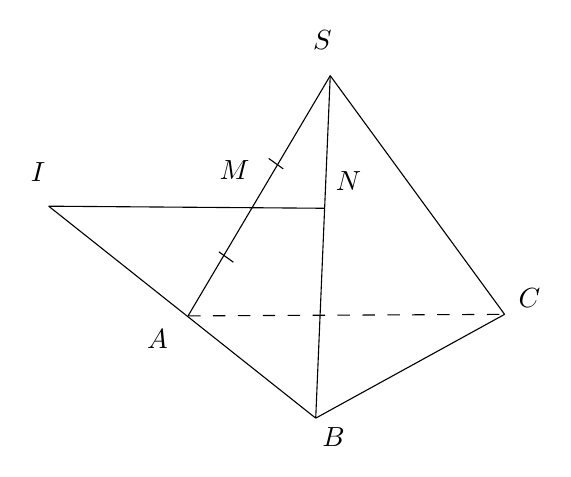
\begin{tikzpicture}[x=0.75pt,y=0.75pt,yscale=-1,xscale=1]
					\draw [dash pattern={on 4.5pt off 4.5pt}] (224,161) -- (376.51,160.26); 
					\draw  (156.86,108.14) -- (285.51,210.26);
					\draw (376.51,160.26) --  (285.51,210.26);
					\draw (292.51,45.26)  -- (376.51,160.26);
					\draw  (292.51,45.26) -- (285.51,210.26);
					\draw  (292.51,45.26) -- (224,161);
					\draw  (156.86,108.14) -- (289.86,109.14);
					\draw (262.86,85.14) --  (269.86,90.14);
					\draw  (238.86,130.14) -- (245.86,135.14);
					\draw (283,22.4) node [anchor=north west][inner sep=0.75pt]  {$S$};
					\draw (287.51,213.66) node [anchor=north west][inner sep=0.75pt] {$B$}; 
					\draw (382,146.4) node [anchor=north west][inner sep=0.75pt] {$C$}; 
					\draw (203,166.4) node [anchor=north  west][inner sep=0.75pt] {$A$};
					 \draw (147,86) node [anchor=north west][inner sep=0.75pt] [align=left] {$I$};
					\draw (238,85) node [anchor=north west][inner  sep=0.75pt] [align=left] {$M$};
					\draw (294,90) node [anchor=north west][inner  sep=0.75pt] [align=left] {$N$};
				\end{tikzpicture}
		\end{center}
		 Trong $\left(SAB\right)$,$ MN\cap AB=\left\{ I\right\}\Rightarrow
		\heva{&I\in MN\\& 
		 I\in AB\Rightarrow I\in\left(ABC\right)}$
		$\Rightarrow  MN\cap\left(ABC\right)=\left\{ I\right\}$.\\
	Vậy giao điểm của $  MN$ với $\left(ABC\right)$ là giao điểm của $ MN$ với $ AB$.}
\end{ex}

% nguồn: Ok_TracNghiemLop11_Lan1
\begin{ex}%[1H4H2-4]%[ma:eac93499]
	Cho tứ diện $ ABCD$. Lấy điểm $ M$ sao  cho $ AM=2CM$ và $ N$ là trung điểm $ AD$. Gọi $ O$ là một điểm thuộc miền trong của $\triangle BCD$. Giao điểm của $ BC$ với $\left(OMN\right)$ là giao điểm của $ BC$ với
	\choice 
		{$OM$} 
		{$MN$} 
		{$OM,MN$  đều đúng}
		{\True  $OM,MN$ đều sai}
	 \loigiai{
		\begin{center}
			\tikzset{every picture/.style={line width=0.75pt}} 
			\begin{tikzpicture}[x=0.75pt,y=0.75pt,yscale=-1,xscale=1]
					\draw [dash pattern={on 4.5pt off 4.5pt}] (231.51,183.01)  -- (435.21,182.15);
					 \draw (231.51,183.01) -- (313.67,239.88);
					 \draw (435.21,182.15) -- (313.67,239.88);
					 \draw (323.02,49.37) -- (435.21,182.15);
					 \draw (323.02,49.37) -- (313.67,239.88);
					 \draw (323.02,49.37) -- (231.51,183.01);
					\draw (273.31,121.16)  -- (317.92,169.97);
					\draw [dash pattern={on 4.5pt off 4.5pt}] (273.31,121.16)  -- (285.77,201.03);
					\draw  [dash pattern={on 4.5pt off 4.5pt}] (317.92,169.97) -- (285.77,201.03);
					\draw (203.49,174.61) node [anchor=north west][inner sep=0.75pt] {$D$}; 
					 \draw (446.93,165.39) node [anchor=north west][inner sep=0.75pt] {$B$};
					\draw (309.42,244.98) node [anchor=north west][inner  sep=0.75pt] {$C$};
					\draw (317.34,29.29)  node [anchor=north west][inner sep=0.75pt] {$A$};
					\draw (257.5,105.82) node [anchor=north west][inner sep=0.75pt] [align=left]  {N};
					\draw (282.22,199.81)  node [anchor=north west][inner sep=0.75pt] [align=left] {O};
					\draw (323.31,153.16) node [anchor=north west][inner sep=0.75pt]  [align=left] {M};
				\end{tikzpicture}
		\end{center}
	Dễ thấy $ OM$ không đồng phẳng với $  BC$ và $ MN$ cũng không đồng phẳng với $ BC$. Vậy cả $OM$ và $MN$ đều sai.}
\end{ex}

% nguồn: Ok_Toan11_TracNghiem_Lan2
\begin{ex}%[1H4V2-4]%[ma:e7f60867]
	Cho hình chóp $S.ABCD$ có đáy $ABCD$ là một hình thang với đáy $AD$ và $BC$. Biết $AD=a$, $BC=b$. Gọi $I$  và $J$ lần lượt là trọng tâm các tam giác $SAD$ và $SBC$. Mặt phẳng $(ADJ)$ cắt $SB$, $SC$ lần lượt tại $M$, $N$. Mặt phẳng $(BCI)$ cắt $SA$, $SD$ tại $P$, $Q$. Khẳng định nào sau đây là đúng?
	 \choice
		{\True  $MN$ song sonng với $PQ$}
		{$MN$ chéo với $PQ$} 
		{$MN$  cắt với $PQ$}
		 {$MN$ trùng với $PQ$}
	\loigiai{ 
		\begin{center}
			\begin{tikzpicture}[scale=.8,line cap=round,line join=round,>=triangle 45,x=1cm,y=1cm]
					 \draw
						 (-3,1)--(-2,-2)--(2,-2)--(6,1)
						 (-1,4.6)--(-3,1)
						 (-1,4.6)--(-2,-2)
						 (-1,4.6)--(2,-2)
						(-1,4.6)--(6,1) 
						 (-1,4.6)--(0,-2)
						(-1.67,0.19)--(1,0.19); 
					 \draw[dashed]
						 (6,1)--(-3,1)
						 (-3,1)--(-0.33,0.19)
						 (-0.33,0.19)--(6,1)
						 (-2,-2)--(0.67,2.19)
						 (0.67,2.19)--(2,-2)
						 (-1,4.6)--(1.5,1)
						 (-2.33,2.19)--(3.67,2.19);
					\begin{scriptsize}
						\foreach \p/\pos/\name in  {
						 (-3,1)/above left/$A$,
						(-2,-2)/below  left/$B$,
						(2,-2)/below right/$C$, 
						(6,1)/above right/$D$, 
						(-1,4.6)/above/$S$} 
						\draw[fill=blue] \p circle  (1pt) node[\pos]{\name};
						\foreach \p/\pos/\name  in {
						(1.5,1)/above  right/$F$,
						(0,-2)/below/$G$, 
						(0.67,2.2)/above/$I$, 
						(-0.33,0.19)/below right/$J$, 
						(-2.33,2.2)/above/$P$, 
						 (3.67,2.2)/above/$Q$,
						(-1.67,0.19)/below  right/$M$,
						(1,0.19)/below  left/$N$}
						\draw[fill] \p circle (1pt)  node[\pos]{\name};
					\end{scriptsize}
				\end{tikzpicture}
		\end{center}
		Ta có $\heva{&MN=(ADJ)\cap (SBC)\\&AD\subset (JAD);BC\subset (SBC)\\& AD\parallel  BC}\Rightarrow MN\parallel AD\parallel BC$.\\
		Tương tự: $\heva{&PQ=(IBC)\cap (SAD)\\& AD\subset (SAD)\\&BC\subset (IBC)\\&AD\parallel BC}\Rightarrow PQ\parallel AD\parallel BC$.\\ 
		 Vậy $MN\parallel PQ$.
	 }
\end{ex}

% nguồn: Ok_Toan11_TracNghiem_Lan2
\begin{ex}%[1H4V2-4]%[ma:4c919af1]
	Cho hình chóp $S.ABCD$ có đáy  $ABCD$ là hình bình hành. Gọi $M$, $N$, $P$ lần lượt là trung điểm của $SB$, $SD$ và $BC$. Gọi $E$ là giao điểm của $(MNP)$ với cạnh $SA$. Tính tỉ số $\dfrac{SE}{SA}$.
	 \choice
		{\True  $\dfrac{1}{4}$}
		{$\dfrac{1}{2}$} 
		{$\dfrac{1}{3}$} 
		 {$\dfrac{3}{4}$}
	\loigiai{ 
		\begin{center}
			\begin{tikzpicture}[scale=1,font=\footnotesize,line join=round,line cap=round,>=stealth]
					\coordinate[label=below  left:$A$] (A) at (0,0);
					\coordinate[label=below:$D$]  (D) at (-20:3);
					\coordinate[label=below:$B$] (B)  at (4,0);
					\coordinate[label=right:$C$] (C)  at ($(B)-(A)+(D)$);
					\coordinate[label=below:$O$] (O)  at ($(A)!.5!(C)$);
					\coordinate[label=above:$S$]  (S) at ($(O)+(90:4)$);
					 \coordinate[label=right:$M$] (M) at ($(S)!0.5!(B)$);
					 \coordinate[label=above left:$N$] (N) at ($(S)!0.5!(D)$);
					\coordinate[label=above right:$P$]  (P) at ($(B)!0.5!(C)$);
					\coordinate[label=below:$K$] (K) at ($(C)!0.5!(D)$); 
					\coordinate[label=above:$I$] (I)  at (intersection of A--C and K--P);
					\coordinate[label=below:$J$] (J) at (intersection of M--N and S--O); 
					\coordinate[label=left:$E$] (E) at (intersection  of I--J and S--A);
					\draw (A)--(D)--(C)--(S)--cycle (S)--(D); 
					\draw[dashed]  (D)--(B)--(A)--(O)
						(S)--(O)--(C)--(B)--cycle  (M)--(N)--(P)--cycle (K)--(P)
						 (I)--(E);
					\foreach \diem in {A,D,C,B,O,S,M,N,P,K,I,J,E} \fill  (\diem) circle (1pt);
				\end{tikzpicture}
		\end{center}
		Mặt phẳng $(MNP)$ song song với  $BD$ nên cắt $DC$ tại trung điểm $K$ của cạnh $DC$.\\
		Kẻ $KP$ cắt $AC$ tại $I$,  kẻ $MN$ cắt $SO$ tại $J$.\\
		Trong mặt phẳng $(SAC)$, kẻ  $IJ$ cắt $SA$ tại $E$.\\
		Do $SC\parallel (MNP)$ nên  $IJ\parallel SC$.\\
		Suy  ra $\dfrac{SE}{SA}=\dfrac{IC}{AC}=\dfrac{1}{4}$.
	} 
\end{ex}


%%%%%%%%%%%%%%%% ĐÚNG/SAI %%%%%%%%%%%%%%%%

% nguồn: Ok_dungsai_lop11_Lan2
\begin{ex}%[1H4H2-4]%[ma:7922345e]
	Cho tứ diện $ABCD$ có $I$, $J$ theo thứ tự là trung điểm của các cạnh $BC$, $BD$. Gọi $(P)$  là mặt phẳng qua $I$, $J$ và cắt các cạnh $AC$, $AD$ lần lượt tại hai điểm $M$, $N$. Khi đó
	\choiceTF 
		{\True $IJ \parallel CD$, $IJ=\dfrac{1}{2}CD$} 
		{$MN$ cắt $DC$} 
		{\True $IJNM$  là một hình thang}
		 {\True Để $IJNM$ là hình bình hành thì $M$ là trung điểm của đoạn $AC$}
	 \loigiai{
		\begin{center}
			\begin{tikzpicture}[scale=1,dot/.style={circle,fill=blue,inner sep=1pt}]
					\coordinate (A) at  (0,3.5);
					\coordinate (B) at (-2.5,0); 
					\coordinate (C) at (0,-1); 
					\coordinate (D) at (3,0.2); 
					\coordinate (M) at ($(A)!0.365!(C)$); 
					\coordinate (N) at ($(A)!0.365!(D)$); 
					\coordinate (I)  at ($(C)!0.5!(B)$);
					\coordinate (J)  at ($(B)!0.5!(D)$);
					 \draw [dashed] (B) -- (D)
						(I) --  (J)--(N);
					\draw  (A) -- (B)
						(A)  -- (C)
						 (A) -- (D)
						 (B) -- (C) -- (D)
						(M)  -- (C)
						(N)--(M)--(I); 
					\node[dot,label=above:$A$] at  (A) {};
					\node[dot,label=left:$B$] at (B) {}; 
					 \node[dot,label=below:$C$] at (C) {};
					\node[dot,label=right:$D$] at (D) {}; 
					\node[dot,label=above left:$M$] at  (M) {};
					\node[dot,label=above  right:$N$] at (N) {};
					\node[dot,label=below left:$I$] at  (I) {};
					 \node[dot,label=below:$J$] at (J) {};
				\end{tikzpicture}
		\end{center}
		\begin{itemchoice}
			\itemch Ta có $IJ$ là đường  trung bình của tam giác $BCD$ nên $IJ\parallel CD$, $IJ=\dfrac{1}{2}CD$.
			\itemch Khi đó $\heva{&(P)\cap  (ACD)=MN\\&IJ\subset (P), CD\subset (ACD)\Rightarrow MN\parallel IJ\parallel CD\\&IJ\parallel CD}$ nên $MN$ song song với $CD$.
			\itemch Khi đó $\heva{&(P)\cap (ACD)=MN\\&IJ\subset (P), CD\subset (ACD)\Rightarrow MN\parallel IJ\parallel CD\\&IJ\parallel  CD}$ vì vậy $IJNM$ là một hình thang.
			\itemch Ta có $IJ\parallel MN$ vì vậy  $IJNM$ là hình bình hành khi và chỉ khi $IJ=MN$.\\
			 Khi đó $MN=\dfrac{1}{2}CD$, $MN\parallel CD$.\\
			Suy ra $MN$ là đường trung bình của tam giác $ACD$ hay  $M$ là trung điểm của đoạn $AC$.
		\end{itemchoice}
	 }
\end{ex}

% nguồn: Ok_dungsai_lop11_Lan1
\begin{ex}%[1H4V2-4]%[ma:aa832a7c]
 Cho hình chóp $S.ABCD$, có đáy $ABCD$ là một hình bình hành tâm  $O$. Gọi $I$, $K$ lần lượt là trung điểm của $SB$ và $SD$. Khi đó:
  \choiceTF
  {\True $SO$ là giao tuyến của $(SAC)$ và $(SBD)$} 
  {Giao điểm $J$ của $SA$ với $(CKB)$ thuộc đường thẳng đi  qua $K$ và song song với $DC$}
  {\True  Giao tuyến của $(OIA)$ và $(SCD)$ là đường thẳng đi qua $C$ và song song với $SD$}
  {\True $CD\parallel IJ$} 
 \loigiai{ 
  \begin{center}
   \begin{tikzpicture}[line join=round,line cap=round,>=stealth,scale=0.85,font=\footnotesize]
     \foreach  \x/\y/\n in {0/0/A,-2/-2/B,6/0/D} \coordinate (\n) at (\x,\y);
     \coordinate (C) at  ($(B)+(D)-(A)$);
      \coordinate (S) at ($(A)+(1,4)$);
     \coordinate (O) at ($(B)!0.5!(D)$); 
     \coordinate (I) at ($(S)!0.5!(B)$); 
     \coordinate  (K) at ($(S)!0.5!(D)$);
     \coordinate (J) at ($(S)!0.5!(A)$); 
     \coordinate  (C1) at ($(C)+(I)-(O)+(I)-(O)$);
      \draw (S)--(D)--(C)--(B)--(S)--(C)--(K);
     \draw[dashed]  (S)--(A)--(D)--(B)--(A)--(C)
      (S)--(O) 
       (A)--(I)--(O)
       (K)--(B)
      (I)--(J)--(K); 
     \draw (K)--($(K)+(0:2)$) coordinate (K1) node[above  left]{$x$};
     \draw (C)--(C1)  node[right]{$y$};
     \foreach \t/\g in  {A/190,B/-150,C/-30,D/30,S/90,I/160,K/60,O/-90,J/150}{
      \draw[fill=black] (\t)  circle (1pt) node[shift={(\g:7pt)}]{$ \t $};
      }
    \end{tikzpicture}
  \end{center}
  \begin{itemchoice}
   \itemch Đúng. Ta có $\heva{&O \in AC \subset(SAC) \\&O \in BD \subset(SBD)} \Rightarrow O \in(SAB)  \cap(SCD)$.\\
    Suy ra $SO=(SAC) \cap(SBD)$.
   \itemch Sai. Tứ giác $ABCD$  là hình bình hành nên $AB \parallel CD$; $AD\parallel BC$.\\
   Ta có $\heva{&AD \parallel CB \\& AD \subset(SAD) \\& BC \subset(SBC) \\ &K  \in(KBC) \cap(SAD)} \Rightarrow\heva{&Kx=(KBC) \cap(SAD) \\& Kx\parallel AD \parallel BC.}$\\
   Trong $(SAD)$ gọi $J=Kx \cap  SA\Rightarrow\heva{&J \in SA \\& J \in Kx \subset(BKC)} \Rightarrow J=SA \cap(BKC)$.
   \itemch Đúng. Ta có $OI$ là đường trung bình của $\triangle SBD \Rightarrow OI \parallel  SD$.\\
   Khi đó $\heva{&OI  \parallel SD \\& OI \subset(OIA) \\& SD \subset(SCD) \\& C \in(OIA) \cap(SCD)} \Rightarrow\heva{&Cy=(OIA) \cap(SCD) \\& Cy \parallel SD \parallel OI.}$
    \itemch Đúng. Ta có
   $\heva{&IJ \parallel AB \text{ ($IJ$ là đường trung bình của $\triangle SAB$)}\\&AB \parallel  CD\text{ (tứ giác $ABCD$ là hình bình hành)}} \Rightarrow CD \parallel IJ$.
  \end{itemchoice}
 } 
\end{ex}

% nguồn: Ok_dungsai_lop11_Lan1
\begin{ex}%[1H4V2-4]%[ma:64d5a36e]
 Cho hình chóp $S.ABCD$ có đáy là hình bình hành, $AC$ và $BD$ cắt nhau tại $O$. Gọi $I$ là trung điểm $SO$. Mặt phẳng $(ICD)$ cắt $SA$, $SB$ lần lượt tại $M$, $N$. Khi  đó:
  \choiceTF
  {\True Điểm $M$ là giao điểm của đường  thẳng $SA$ với mặt phẳng $(ICD)$}
  {Ta có  $SN=\dfrac{2}{3}SB$}
  {Cho  $AB=a$ thì $MN=\dfrac{a}{2}$}
  {Trong mặt phẳng $(CDMN)$, gọi $K$ là giao điểm của $CN$ và $DM$. Khi đó $SK$ và $BC$ chéo  nhau}
  \loigiai{
  \begin{center}
   \begin{tikzpicture}[line join=round,line cap=round,>=stealth,scale=0.85,font=\footnotesize]
     \foreach \x/\y/\n in {0/0/A,-2.5/-2/B,6/0/D} \coordinate (\n) at (\x,\y); 
     \coordinate  (C) at ($(B)+(D)-(A)$);
     \coordinate  (S) at ($(A)+(1,4)$);
     \coordinate (O) at ($(B)!0.5!(D)$); 
      \coordinate (I) at ($(S)!0.5!(O)$);
     \coordinate  (M) at ($(S)!1/3!(A)$);
     \coordinate  (N) at ($(S)!1/3!(B)$);
     \coordinate  (E) at ($(S)!2/3!(B)$);
     \coordinate (K) at ($(D)!3/2!(M)$); 
     \draw  (S)--(B)--(C)--(D)--(S)--(C)--(K)--(S);
     \draw[dashed]  (S)--(A)--(D)--(B)
       (C)--(A)--(B)
       (M)--(C)
      (S)--(O)--(E) 
      (N)--(D)--(M)--(N) 
      (M)--(K); 
      \foreach \t/\g in {A/150,B/-150,C/-30,D/30,S/90,O/-90,M/30,N/170,E/170,I/40,K/150}{
      \draw[fill=black] (\t) circle (1pt) node[shift={(\g:7pt)}]{$ \t  $};
      }
    \end{tikzpicture}
  \end{center}
  \begin{itemize}
   \item  Xác định $M$, $N$:\\
   Trong mặt phẳng $(SAC)$, kẻ $CI$ cắt  $SA$ tại $M$;\\
   Trong mặt phẳng $(SBD)$,  kẻ $DI$ cắt $SB$ tại $N$.\\
   Vì $\heva{&M \in CI,  CI \subset(ICD) \\& M \in SA} \Rightarrow M=SA \cap(ICD)$.\\
   Tương tự $\heva{&N \in DI, DI \subset(ICD) \\& N \in SB} \Rightarrow  N=SB \cap(ICD)$.
   \item Tính $MN$ theo  $a$:\\
   Gọi $E$ là trung điểm $BN$,  $OE$ là đường trung bình của tam giác $BDN\Rightarrow OE \parallel DN$.\\
   Trong tam giác $SOE$, ta có $NI$ qua trung điểm $I$ của $SO$ và $NI \parallel  OE$, $N$ là trung điểm của $SE$.\\
   Vậy $SN=NE=EB$  hay $SN=\dfrac{1}{3} SB$.\\
   Hoàn toàn tương tự, ta chứng minh  được $SM=\dfrac{1}{3} SA$.\\
   Khi đó  hai tam giác $SMN$, $SAB$ đồng dạng vì có góc $S$ chung và $\dfrac{SM}{SA}=\dfrac{SN}{SB}=\dfrac{1}{3}$.\\
   Xét tam giác $SAB$, theo  định lí Thalès, ta có
    $\dfrac{MN}{AB}=\dfrac{SM}{SA}=\dfrac{1}{3} \Rightarrow MN=\dfrac{AB}{3}=\dfrac{a}{3}$.
   \item Chứng minh $SK \parallel BC \parallel  AD$:\\
   Dễ thấy  $S$ là điểm chung của hai mặt phẳng $(SBC)$ và $(SAD)$.\\
   Ta có $\heva{&K \in CN, CN \subset(SBC) \\& K  \in DM, DM \subset(SAD)} \Rightarrow K \in(SBC) \cap(SAD)$.\\
   Vì  vậy $SK=(SBC) \cap(SAD)$.\\
   Khi đó $\heva{&SK=(SBC) \cap(SAD) \\& BC \subset(SBC), AD \subset(SAD) \\& BC \parallel AD}\Rightarrow  SK \parallel BC \parallel AD$.
  \end{itemize}
  \begin{itemchoice}
   \itemch  Đúng.
   \itemch  Sai.
    \itemch Sai.
   \itemch  Sai.
  \end{itemchoice}
  }
\end{ex}

% nguồn: Ok_dungsai_lop11_Lan2
\begin{ex}%[1H4V2-4]%[ma:a3aa1f52]
	Cho hình chóp $S.ABCD$ có đáy $ABCD$ là hình bình hành tâm $O$. Gọi $M$, $N$ lần lượt  là trung điểm của $SC$ và $OB$.
	 \choiceTF
		{Giao điểm của $SC$ và  mặt phẳng $(AMN)$ là điểm $N$}
		{\True Giao điểm của $AM$ và mặt phẳng $(SBD)$ là trọng tâm  của tam giác $SAC$}
		{Giao điểm của $NI$ và mặt phẳng $(SAD)$ là điểm $K$ thuộc đường thẳng $SA$} 
		{Giao điểm của đường thẳng $SD$ và mặt phẳng $(AMN)$ là trung điểm  của $SD$}
	\loigiai{ 
		\begin{center}
			\begin{tikzpicture}[scale=0.8,font=\footnotesize,line join=round,line cap=round,>=stealth]
					 \def\a{4}
					\coordinate (A) at  (0,0);
					\coordinate (B) at  (\a*1.3,0);
					\coordinate  (D) at ($(A)+(\a*0.4,\a*0.5)$);
					\coordinate (C) at  ($(B)+(D)-(A)$);
					 \coordinate (S) at ($(\a*0.6,\a*1.5)$);
					\coordinate (O)  at ($(A)!0.5!(C)$);
					\coordinate (M)  at ($(S)!0.5!(C)$);
					\coordinate (N)  at ($(O)!0.5!(B)$);
					\coordinate (K) at  ($(S)!0.4!(D)$);
					 \coordinate (I) at ($(S)!2/3!(O)$);
					 \draw (S)--(B)--(C)--(S)--(A)--(B);
					\draw[dashed]  (B)--(D)--(A)--(C)
						 (O)--(S)--(D)--(C)
						 (M)--(N)--(A)--(M)
						 (N)--(K);
					\foreach  \x/\label/\g in {K/\(K\)/10,S/\(S\)/90,B/\(B\)/-90,C/\(C\)/-80,D/\(D\)/140,A/\(A\)/-90,O/\(O\)/-90,M/\(M\)/20,N/\(N\)/20,I/\(I\)/-10}
					\fill (\x) circle (1pt) 
						 ($(\x)+(\g:3mm)$) node{\small $\x$};
					\fill[cyan!50,opacity=0.3]  (A)--(M)--(N);
				\end{tikzpicture}
		\end{center}
		\begin{itemchoice}
			\itemch  \textbf{Sai} \\
			Dễ thấy giao điểm của $SC$  và mặt phẳng $(AMN)$ là điểm $M$.
			\itemch \textbf{Đúng}  \\
			Trong mặt phẳng $(SAC)$, gọi $I  = AM \cap SO$:
			 \[
			\heva{&I  \in AM \\ &I \in SO, SO \subset (SBD)}
			\Rightarrow I = AM \cap (SBD). 
			\] 
			Do $AM$, $SO$ là hai đường trung tuyến trong tam giác $SAC$, nên $I$ là trọng tâm của tam  giác $SAC$.
			\itemch  \textbf{Sai}\\
			Trong mặt phẳng $(SBD)$, gọi  $K = NI \cap SD$.\\
			Ta  có
			\[ 
			\heva{&K \in NI \\&K  \in SD, SD \subset (SAD)}
			\Rightarrow K = NI \cap  (SAD).
			 \]
			Vậy giao điểm  của $NI$ và mặt phẳng $(SAD)$ là điểm $K$ thuộc đường thẳng $SD$.
			\itemch \textbf{Sai}  \\
			Ta có: 
			 \[
			 \heva{&K \in SD \\ &K \in NI, NI \subset (AMN)}
			\Rightarrow K = SD  \cap (AMN).
			 \]
			Ta có $I$  là trọng tâm tam giác $SAC$ suy ra $I$ là trọng tâm tam giác $SBD$.\\
			Nếu $K$ là trung điểm của $SD$ thì do $I$ là trọng tâm tam giác $SBD$ suy ra $KI$ chính là trung tuyến thứ hai của tam giác  $SBD$.\\
			Vì thế $KI$ đi qua $B$. Điều này là vô lý.\\ 
			 Vậy $K$ không là trung điểm của $SD$.
		\end{itemchoice}
	} 
\end{ex}

% nguồn: Ok_dungsai_lop11_Lan2
\begin{ex}%[1H4V2-4]%[ma:4c468b65]
	Cho  tứ giác $ABCD$ có $AC$ và $BD$ giao nhau tại $O$ và một điểm $S$ không thuộc mặt phẳng $(ABCD)$. Trên đoạn $SC$ lấy một điểm $M$ không trùng với $S$ và $C$, $K=AM\cap SO$. Khi đó
	\choiceTF 
		{$S O$ là giao tuyến  của hai mặt phẳng $(SAC)$ và $(ABC)$}
		{\True $SO$ là giao tuyến của  hai mặt phẳng $(SAC)$ và $(SBD)$}
		{\True Giao điểm của đường thẳng $SO$ với  mặt phẳng $(ABM)$ là điểm $K$}
		{Giao điểm của  đường thẳng $SD$ với mặt phẳng $(ABM)$ là điểm $N$ thuộc đường thẳng $AK$}
	 \loigiai{
		\begin{center}
			\begin{tikzpicture}[scale=1,font=\footnotesize,line join=round,line cap=round,>=stealth]
					\coordinate  (A) at (0,0);
					\coordinate (B)  at (1,-2);
					\coordinate (C)  at (3.5,-1.5);
					\coordinate (D) at (5,0); 
					\path[name path=AC]  (A)--(C);
					\path[name  path=BD] (B)--(D);
					\path[name intersections={of=AC and BD,by=O}]; 
					\coordinate (S)  at (2,4.2);
					\coordinate (M) at ($(S)!0.55!(C)$); 
					 \path[name path=SO] (S)--(O);
					\path[name path=AM]  (A)--(M);
					\path[name  intersections={of=SO and AM,by=K}];
					 \draw (A)--(B)--(C)--(D);
					\draw[dashed] (D)--(A) 
						(A)--(C) 
						(B)--(D) 
						 (S)--(O)
						 (A)--(M);
					\draw (S)--(A) 
						(S)--(B) 
						(S)--(C) 
						 (S)--(D)
						(S)--(C); 
					\foreach \p in {A,B,C,D,S,O,M,K} 
					 \fill (\p) circle (1pt);
					 \node[below left] at (A) {$A$};
					\node[below] at (B)  {$B$};
					\node[below  right] at (C) {$C$};
					\node[above right] at (D)  {$D$};
					 \node[above] at (S) {$S$};
					\node[below] at (O) {$O$}; 
					\node[above right] at (M)  {$M$};
					\node[above  left] at (K) {$K$};
				\end{tikzpicture}
		\end{center}
		\begin{itemchoice}
			 \itemch
			Điểm  $S$ không thuộc mặt phẳng $(ABC)$ nên $SO$ khôg phải là giao tuyến của hai mặt phẳng $(SAC)$ và $(ABC)$.
			\itemch Ta có $S\in(SAC)\cap (SBD)$, $O\in (SAC)\cap (SBD)$ nên $S O$ là giao tuyến của hai mặt phẳng $(SAC)$ và  $(SBD)$.
			\itemch Tìm giao điểm của $SO$  và $(ABM)$.\\
			Trong mặt phẳng $(SAC)$ gọi  $K=AM\cap SO$.\\
			Vì $\heva{&K\in AM,\,AM  \subset(ABM)\\ &K \in SO}\Rightarrow K=SO\cap(ABM)$.
			\itemch Tìm giao điểm của  $SD$ và $(ABM)$. Xét mặt phẳng phụ $(SBD)$ chứa $SD$.\\
			Dễ thấy $B$ là điểm chung của hai mặt phẳng $(SBD)$  và $(ABM)$.\\
			Ta có $\heva{&K\in AM,\,AM\subset(ABM)\\ &K\in  SO,\,SO\subset(SBD).}$\\
			Suy  ra $K\in(SBD)\cap(ABM)$. Do đó $BK=(SBD)\cap(ABM)$.\\
			 Trong mặt phẳng $(SBD)$ gọi $N=BK\cap SD$.\\
			Do $\heva{&N\in SD\\&N\in  BK,\,BK\subset(ABM)}\Rightarrow N=SD\cap(ABM)$.
		\end{itemchoice}
	} 
\end{ex}

% nguồn: Ok_dungsai_lop11_Lan2
\begin{ex}%[1H4V2-4]%[ma:34459895]
	Cho hình chóp $S.ABCD$ có đáy $ABCD$ là một hình thang với đáy lớn $AD$. Gọi $I$ và $J$ lần lượt là trọng tâm các tam giác $SAD$ và $SBC$. Mặt phẳng $(ADJ)$ cắt $SB$, $SC$ lần lượt tại $M$, $N$. Mặt phẳng $(BCI)$ cắt $SA$, $SD$ tại $P$, $Q$. Khi  đó
	 \choiceTF
		{\True Hai đường thẳng $AD$ và $BC$ song  song với nhau}
		{\True Điểm $I$ nằm trên đường thẳng $PQ$} 
		{Hai đường thẳng  $MN$ và $BC$ chéo nhau}
		{\True Hai đường thẳng $MN$ và $PQ$ song song với nhau} 
	\loigiai{\begin{center}
		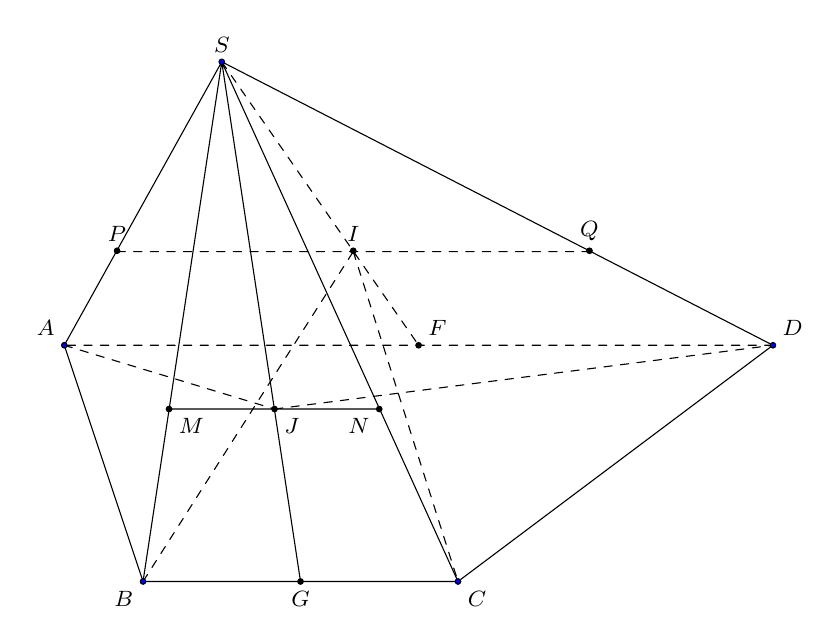
\begin{tikzpicture}[scale=1,font=\footnotesize,line join=round,line cap=round,>=stealth]
				 \draw
					(-3,1)--(-2,-2)--(2,-2)--(6,1) 
					 (-1,4.6)--(-3,1)
					(-1,4.6)--(-2,-2) 
					(-1,4.6)--(2,-2) 
					 (-1,4.6)--(6,1)
					(-1,4.6)--(0,-2) 
					 (-1.67,0.19)--(1,0.19);
				\draw[dashed] 
					(6,1)--(-3,1) 
					(-3,1)--(-0.33,0.19) 
					 (-0.33,0.19)--(6,1)
					(-2,-2)--(0.67,2.19) 
					(0.67,2.19)--(2,-2) 
					(-1,4.6)--(1.5,1) 
					 (-2.33,2.19)--(3.67,2.19);
				\foreach \p/\pos/\name in  {
					 (-3,1)/above left/$A$,
					(-2,-2)/below left/$B$, 
					 (2,-2)/below right/$C$,
					(6,1)/above right/$D$, 
					(-1,4.6)/above/$S$} 
				\draw[fill=blue]  \p circle (1pt) node[\pos]{\name};
				 \foreach \p/\pos/\name in {
					(1.5,1)/above right/$F$, 
					(0,-2)/below/$G$, 
					 (0.67,2.2)/above/$I$,
					(-0.33,0.19)/below  right/$J$,
					 (-2.33,2.2)/above/$P$,
					(3.67,2.2)/above/$Q$, 
					(-1.67,0.19)/below right/$M$, 
					 (1,0.19)/below left/$N$}
				 \draw[fill] \p circle (1pt) node[\pos]{\name};
			\end{tikzpicture}
	\end{center}
	\begin{itemchoice}
		\itemch Ta có $I\in (SAD) \Rightarrow I\in (SAD) \cap (IBC)$ nên $\heva{&AD\subset (SAD) \\&BC\subset  (IBC) \\&AD\parallel BC\\& (SAD) \cap (IBC)=PQ.}$
		\itemch Ta có  $PQ\parallel AD\parallel BC\ (1)$ và $I\in PQ$.
		\itemch Tương tự $J\in  (SBC) \Rightarrow J\in (SBC) \cap (ADJ)$ nên $\heva{&AD\subset (ADJ) \\&BC\subset (SBC) \\&AD\parallel BC\\& (SBC) \cap (ADJ)=MN.}$
		\itemch Ta có $MN\parallel AD\parallel BC$ và  $J\in MN$ suy ra $MN\parallel PQ$.
	\end{itemchoice}
} 
\end{ex}

% nguồn: Ok_dungsai_lop11_Lan2
\begin{ex}%[1H4V2-4]%[ma:23298af2]
	Cho hình chóp $S.ABCD$ có đáy là hình bình hành, $AC$ và $BD$ cắt  nhau tại $O$. Gọi $I$ là trung điểm của đoạn thẳng $SO$. Mặt phẳng $(ICD)$ cắt $SA$, $SB$ lần lượt tại $M$, $N$. Hai đường thẳng $CN$ và $DM$ cắt nhau tại $K$.
	\choiceTF 
		{\True Điểm $M$ là giao điểm  của đường thẳng $SA$ với mặt phẳng $(ICD)$}
		{$SN = \dfrac{2}{3}SB$} 
		{$MN  = \dfrac{AB}{2}$}
		{$SK$ và $BC$  chéo nhau}
	\loigiai{ 
		\begin{center}
			\begin{tikzpicture}[scale=0.8,font=\footnotesize,line join=round,line cap=round,>=stealth]
					\def\a{4} 
					\def\b{1/3} 
					\coordinate (B) at  (0,0);
					\coordinate  (C) at (\a*1.2,0);
					\coordinate  (A) at ($(B)+(\a*0.45,\a*0.5)$);
					\coordinate (D) at  ($(A)+(C)-(B)$);
					\coordinate  (S) at ($(\a*0.85,\a*1.6)$);
					 \coordinate (O) at ($(A)!0.5!(C)$);
					\coordinate (I) at ($(S)!0.5!(O)$); 
					\coordinate (M)  at ($(S)!1/3!(A)$);
					 \coordinate (N) at ($(S)!1/3!(B)$);
					\coordinate (K)  at ($(D)!1.5!(M)$);
					\coordinate (E)  at ($(N)!0.5!(B)$);
					\draw  (S)--(B)--(C)--(D)--(S)--(C)--(K)--(S);
					\draw[dashed] (N)--(B)--(A)--(D)--(B); 
					\draw[dashed] (C)--(A)--(S)--(O)--(E); 
					\draw[dashed]  (C)--(M)--(N)--(D)--(K);
					\foreach \x/\label/\g in  {A/\(A\)/120,B/\(B\)/-90,C/\(C\)/-90,D/\(D\)/-60,S/\(S\)/90,O/\(O\)/-100,I/\(I\)/-130,M/\(M\)/20,N/\(N\)/180,E/\(E\)/180,K/\(K\)/90}
					\fill (\x) circle  (1pt)
						($(\x)+(\g:3mm)$)  node {\small \label};
				\end{tikzpicture}
		\end{center}
		\begin{itemchoice}
			\itemch \textbf{Đúng}  \\
			Trong mặt phẳng $(SAC)$, kẻ $CI$ cắt $SA$ tại $M$; \\ 
			 \[
			\heva{ 
			 &M \in CI, CI \subset (ICD) \\
			&M \in SA 
			} 
			\Rightarrow M = SA \cap  (ICD).
			\] 
			 \itemch \textbf{Sai} \\
			 Trong mặt phẳng $(SBD)$, kẻ $DI$ cắt $SB$ tại $N$. Tương tự
			\[ 
			\heva{ 
			&N \in DI, DI \subset  (ICD) \\
			&N \in SB 
			} 
			\Rightarrow N = SB  \cap (ICD).
			\] 
			Gọi $E$ là trung điểm  $BN$, $OE$ là đường trung bình của tam giác $BDN$ nên $OE \parallel DN$.\\
			Trong tam giác $SOE$, ta có $NI$ đi qua trung điểm $I$  của $SO$ và $NI \parallel OE$, $N$ là trung điểm của $SE$.\\
			 \[
			 \Rightarrow SN = NE = EB \Rightarrow SN = \dfrac{1}{3}SB.
			\] 
			 \itemch \textbf{Sai}\\
			Hoàn toàn  tương tự, ta chứng minh được $SM = \dfrac{1}{3}SA$.\\
			Khi đó hai tam giác $SMN$, $SAB$ đồng dạng vì  có góc $S$ chung và
			$\dfrac{SM}{SA} = \dfrac{SN}{SB} = \dfrac{1}{3}$.\\ 
			Xét tam giác $SAB$, theo định lí  Thales, ta có\\
			 \[
			 \dfrac{MN}{AB} = \dfrac{1}{3} \Rightarrow MN = \dfrac{AB}{3}.
			\] 
			\itemch \textbf{Sai} \\ 
			Ta  có
			\[ 
			 \heva{
			&K \in CN, CN \subset (SBC)  \\
			 &K \in DM, DM \subset (SAD)
			 }
			\Rightarrow K \in (SBC) \cap  (SAD).
			\] 
			 và
			 \[
			\heva{ 
			&S  \in (SBC) \cap (SAD)\\
			&K \in  (SBC) \cap (SAD)
			} 
			\Rightarrow SK =  (SBC) \cap (SAD).
			 \]
			 \[
			\heva{&SK = (SBC)  \cap (SAD) \\&BC \subset (SBC), AD \subset (SAD) \\&BC \parallel AD}
			\Rightarrow SK  \parallel BC.
			 \]
		\end{itemchoice}
	 }
\end{ex}

% nguồn: Ok_dungsai_lop11_Lan2
\begin{ex}%[1H4V2-4]%[ma:90bd95b8]
	Cho hình chóp $S.ABCD$ có đáy là hình bình hành, $AC$ và $BD$ cắt nhau tại $O$. Gọi $I$  là trung điểm $SO$. Mặt phẳng $(ICD)$ cắt $SA$, $SB$ lần lượt tại $M$, $N$.
	\choiceTF 
		{\True Điểm $M$ là giao điểm của  đường thẳng $SA$ với mặt phẳng $(ICD)$}
		{Ta có $SN=\dfrac{2}{3}SB$} 
		{Cho $AB=a$  thì $MN=\dfrac{a}{2}$}
		{Trong mặt phẳng $(CDMN)$, gọi $K$ là giao điểm của $CN$  và $DM$. Khi đó $SK$ và $BC$ chéo nhau}
	\loigiai{ 
		\begin{center}
			\begin{tikzpicture}[scale=1,font=\footnotesize,line join=round,line cap=round,>=stealth]
					 \coordinate[label=above left:$A$] (A) at (0,0);
					\coordinate[label=below:$B$] (B) at  (-150:3);
					\coordinate[label=below:$D$] (D) at (4,0); 
					\coordinate[label=below:$C$] (C)  at ($(D)-(A)+(B)$);
					\coordinate[label=below:$O$] (O) at  ($(A)!.5!(C)$);
					\coordinate[label=above:$S$] (S) at ($(O)+(74:4)$); 
					 \coordinate[label=below left:$I$] (I) at ($(S)!.5!(O)$);
					 \coordinate[label=above:$M$] (M) at ($(S)!1/3!(A)$);
					 \coordinate[label=left:$N$] (N) at ($(S)!1/3!(B)$);
					\coordinate[label=left:$E$] (E)  at ($(S)!2/3!(B)$);
					\coordinate[label=above left:$K$] (K) at (intersection  of C--N and M--D);
					 \draw (B)--(C)--(S)--cycle (C)--(D)--(S)--(B)
						 (S)--(K)--(C);
					\draw[dashed] (B)--(D)--(A)--cycle (C)--(A)--(S)--(O)--(E) 
						 (N)--(M)--(C)
						 (N)--(D)--(K);
					\foreach  \diem in {A,B,C,D,O,S,I,M,N,E,K} \fill (\diem) circle (1pt);
				\end{tikzpicture}
		\end{center}
		\begin{itemchoice}
			\itemch Trong mặt phẳng $(SAC)$  kẻ $CI$ cắt $SA$ tại $M$.\\
			Trong mặt phẳng $(SBD)$ kẻ  $DI$ cắt $SB$ tại $N$.\\
			Ta  có $\heva{
			&M\in CI, CI\subset(ICD)\\ 
			 &M\in SA.
			}$\\ 
			Suy ra $M=SA\cap(ICD)$. 
			\itemch Ta có $\heva{ 
			&N\in  DI, DI\subset(ICD)\\
			&N\in SB. 
			}$\\ 
			Suy ra  $N=SB\cap(ICD)$.\\
			Gọi $E$ là trung điểm $BD$. Khi đó $OE$  là đường trung bình tam giác $BDN$.\\
			Suy ra $OE\parallel DN$.\\ 
			Trong tam  giác $SOE$, ta có $NI$ qua trung điểm $I$ của $SO$ và $N\in SE$.\\
			 Suy ra $NI\parallel OE$.\\
			Mà $OE\parallel DN$  nên $NI\parallel DN$.\\
			 Suy ra $N$ là trung điểm $SE$.\\
			Khi đó, ta có $SN=\dfrac{1}{3}SB$  (do $E$ trung điểm $BD$ và $NE=EB$).\\
			Tương  tự, ta chứng minh được $SM=\dfrac{1}{3}SA$.\\
			Ta lại có tam giác $SMN$ và tam  giác $SAB$ đồng dạng. Ta được \[\dfrac{SM}{SA}=\dfrac{SN}{SB}=\dfrac{1}{3}\Rightarrow SN=\dfrac{1}{3}SB.\]
			\itemch Xét tam giác $SAB$. Theo định lí Thales, ta  được
			\[\dfrac{MN}{AB}=\dfrac{SM}{SA}=\dfrac{1}{3}.\] 
			Suy ra  $MN=\dfrac{AB}{3}=\dfrac{a}{3}$.\\
			\itemch  Dễ thấy $S$ là điểm chung của hai mặt phẳng $(SBC)$ và $(SAD)$.\\
			 Ta có
			$\heva{ 
			&K\in CN,  CN\subset(SBC)\\
			&K\in DM,  DM\subset(SAD).
			 }$\\
			 Suy ra $K\in(SBC)\cap(SAD)$.\\
			 Khi đó, ta có
			\[\heva{ 
			&SK=(SBC)\cap(SAD)\\ 
			 &BC\subset(SBC), AD\subset(SAD)\\
			&BC\parallel  AD.
			 }\]
			 Suy ra $SK\parallel BC\parallel AD$.
		\end{itemchoice}
	} 
\end{ex}

% nguồn: Ok_dungsai_lop11_Lan2
\begin{ex}%[1H4V2-4]%[ma:dcb0d3c7]
	Cho hình chóp $S.ABCD$ có đáy $ABCD$ là  hình thang ($AD$ là đáy lớn, $BC$ là đáy nhỏ). Gọi $E$, $F$ lần lượt là trung điểm của $SA$ và $SD$. Gọi $K$ là giao điểm của các đường thẳng $AB$ và $CD$.
	\choiceTF 
		{\True Giao điểm $M$ của đường thẳng $SB$ và mặt phẳng $(CDE)$ là điểm thuộc  đường thẳng $KE$}
		{Đường thẳng $SC$ cắt mặt phẳng $(EFM)$ tại $N$. Tứ giác $EFNM$ là  hình bình hành}
		{\True Các đường thẳng $AM$, $DN$,  $SK$ cùng đi qua một điểm}
		{Cho biết $AD=2BC$.  Tỉ số diện tích của hai tam giác $KMN$ và $KEF$ bằng $\dfrac{S_{\triangle KMN}}{S_{\triangle KEF}}=\dfrac{2}{3}$}
	 \loigiai{
		\begin{center}
			\begin{tikzpicture}[scale=1,font=\footnotesize,line join=round,line cap=round,>=stealth]
					\coordinate[label=left:$A$] (A)  at (0,0);
					\coordinate[label=right:$D$]  (D) at (4,0);
					\coordinate[label=below:$K$] (K) at  (-60:3);
					\coordinate[label=above:$S$] (S)  at (70:4);
					\coordinate[label=left:$E$] (E) at  ($(A)!.5!(S)$);
					\coordinate[label=right:$F$] (F) at ($(S)!.5!(D)$); 
					\coordinate[label=above right:$I$] (I)  at ($(S)!.5!(K)$);
					\coordinate[label=below  left:$B$] (B) at ($(A)!.5!(K)$);
					\coordinate[label=below  right:$C$] (C) at ($(D)!.5!(K)$);
					\coordinate[label=above left:$M$] (M) at (intersection of S--B  and A--I);
					\coordinate[label=above left:$N$] (N) at (intersection  of S--C and D--I);
					 \draw (A)--(K)--(D)--(S)--cycle (S)--(K)
						 (C)--(S)--(B)
						(A)--(I)--(D) 
						(E)--(K)--(F); 
					 \draw[dashed] (A)--(D)
						 (E)--(F)--(M)
						 (C)--(E)--(D)
						 (M)--(N)
						(B)--(C); 
					\foreach \diem  in {A,K,D,S,E,F,I,B,C,M,N} \fill (\diem) circle (1pt);
				\end{tikzpicture}
		\end{center}
		\begin{itemchoice}
			\itemch Ta có  $SK=(SAB)\cap(SCD)$.\\
			Trong mặt phẳng $(SAB)$ gọi $M=KE\cap SB$ thì  ta có $KE\subset(CDE)$.\\
			Do đó $SB\cap(CDE)=M$. 
			\itemch Trong mặt phẳng  $(SCD)$, gọi $N=KF\cap SC$ thì ta có $KF\subset(EFM)$.\\
			Do  đó $SC\cap(EFM)=N$.\\
			 Khi đó ta có
			$\heva{ 
			 &MN=(EFK)\cap(SBC)\\
			 &EF\parallel BC\\
			&EF\subset(EFK)\\ &BC\subset(SBC). 
			 }$\\
			Suy ra  $MN\parallel EF\parallel BC$.\\
			Vậy tứ giác $EFNM$ là  hình thang.
			\itemch Trong mặt phẳng  $(ADNM)$, gọi $I=AM\cap DN$.\\
			 Mà
			$\heva{ 
			&I\in  AM, AM\subset(SAB)\\
			&I\in CD,  CD\subset(SCD).
			 }$\\
			Suy  ra $I\in(SAB)\cap(SCD)$.\\
			Hay $I\in SK$ nên 3 đường thẳng $AM$, $DN$, $SK$ đồng quy tại điểm $I$. 
			\itemch Ta có $MN=\dfrac{2}{3}EF$.\\ 
			Gọi $h_1$, $h_2$ lần  lượt là các đường cao từ $K$ xuống đoạn thẳng $MN$ và $EF$.\\
			Suy ra  $h_1=\dfrac{2}{3}h_2$.\\
			 Khi đó, ta có
			\[\dfrac{S_{\triangle KMN}}{S_{\triangle KEF}}=\dfrac{\dfrac{1}{2}MN\cdot  h_1}{\dfrac{1}{2}EF\cdot h_2}=\dfrac{\dfrac{2}{3}EF\cdot\dfrac{2}{3}h_2}{EF\cdot h_2}=\dfrac{4}{9}.\]
		\end{itemchoice}
	 }
\end{ex}

% nguồn: Ok_dungsai_lop11_Lan1
\begin{ex}%[1H4C2-4]%[ma:947ab97b]
 Cho hình chóp $S.ABCD$ có đáy $ABCD$ là hình thang ($A D$ là đáy lớn, $BC$ là đáy  nhỏ). Gọi $E$, $F$ lần lượt là trung điểm của $SA$ và $SD$. $K$ là giao điểm của các đường thẳng $AB$ và $CD$. Khi đó:
  \choiceTF
  {\True Giao điểm $M$ của đường thẳng $SB$ và mặt phẳng  $(CDE)$ là điểm thuộc đường thẳng $KE$}
  {Đường thẳng $SC$ cắt mặt phẳng $(EFM)$ tại $N$. Tứ  giác $EFNM$ là hình bình hành}
  {\True Các đường thẳng $AM$, $DN$, $SK$ cùng đi qua  một điểm}
  {Cho biết $AD=2BC$. Tỉ số diện tích của hai tam giác $KMN$ và  $KEF$ bằng $\dfrac{S_{\triangle KMN}}{S_{\triangle KEF}}=\dfrac{2}{3}$}
 \loigiai{ 
  \begin{center}
   \begin{tikzpicture}[line join=round,line cap=round,>=stealth,scale=0.9,font=\footnotesize]
     \foreach \x/\y/\n in {0/0/A,2/-1.5/B,6/0/D} \coordinate (\n)  at (\x,\y);
      \coordinate (C) at ($(B)+(0:3)$);
      \coordinate (S) at ($(A)+(2.5,6)$);
     \coordinate (B1) at  ($(A)!2!(B)$);
     \coordinate  (C1) at ($(D)!2!(C)$);
     \coordinate (E)  at ($(S)!1/2!(A)$);
     \coordinate (F) at ($(S)!1/2!(D)$); 
     \path 
      (intersection of A--C and B--D)  coordinate (O)
      (intersection of A--B1 and D--C1)  coordinate (K)
      (intersection of E--K and S--B) coordinate (M) 
      (intersection of F--K and  S--C) coordinate (N);
     \coordinate  (M1) at ($(A)!2!(M)$);
     \path (intersection of S--K  and A--M1) coordinate (I);
     \draw (S)--(A)--(K)--(D)--(S)--(K) 
      (B)--(S)--(C) 
       (A)--(I)--(D)
      (E)--(K)--(F); 
     \draw[dashed] (A)--(D) 
       (B)--(C)
       (E)--(F)--(M)
      (C)--(E)--(D) 
      (M)--(N); 
     \foreach \t/\g in {A/150,B/-150,C/-30,D/30,S/90,K/-90,M/170,N/-130,E/150,F/30,I/160}{ 
      \draw[fill=black] (\t) circle (1pt) node[shift={(\g:7pt)}]{$ \t  $};
      }
    \end{tikzpicture}
  \end{center}
  \begin{itemize}
   \item Có $SK=(SAB)  \cap(SCD)$.\\
   Trong mp$(SAB)$, gọi $M=KE \cap SB$,  có $KE \subset(CDE)$. Do đó $SB \cap(CDE)=M$.
   \item Trong mp$(SCD)$, gọi $N=KF  \cap SC$, có $KF \subset(EFM)$.\\
   Do  đó $SC \cap(EFM)=N$.\\
   Suy ra $\heva{&MN=(EFK) \cap(SBC) \\& EF \parallel BC; EF \subset(EFK), BC \subset(SBC)}\Rightarrow MN \parallel EF  \parallel BC$.\\
   Suy ra  tứ giác $EFNM$ là hình thang.
   \item Trong mp$(ADNM)$, gọi $I=AM  \cap DN$.\\
   Mà $\heva{&I  \in AM, AM \subset(SAB) \\ &I \in CD, CD \subset(SCD)} \Rightarrow I \in(SAB) \cap(SCD)$.\\
   Hay $I\in SK$. Vậy 3 đường thẳng $AM$, $DN$, $SK$  đồng quy tại điểm $I$.
   \item Khi $AD=2BC$ dễ dàng chứng minh được $B$, $C$ lần lượt là trung điểm của $KA$ và $KD$.  \\
   Suy ra $M$, $N$ lần lượt là trọng tâm  của hai tam giác $SAK$ và $SDK$.\\
   Do đó $MN=\dfrac{2}{3} EF$, gọi $h_1$, $h_2$ lần lượt là độ dài đường cao xuất phát từ đỉnh $K$ xuống hai đáy  $MN$ và $EF$, dễ thấy $h_1=\dfrac{2}{3} h_2$.\\
   Vậy $\dfrac{S_{\triangle KMN}}{S_{\triangle KEF}}=\dfrac{\dfrac{1}{2} MN \cdot h_1}{\dfrac{1}{2}  EF \cdot h_2}=\dfrac{\dfrac{2}{3} EF \cdot \dfrac{2}{3} h_2}{EF \cdot h_2}=\dfrac{4}{9}$.
  \end{itemize}
  \begin{itemchoice}
   \itemch  Đúng.
   \itemch Sai. 
   \itemch  Đúng.
   \itemch Sai. 
  \end{itemchoice}
  }
\end{ex}


%%%%%%%%%%%%%%%% TRẢ LỜI NGẮN %%%%%%%%%%%%%%%%

% nguồn: Ok_TraLoiNgan_Lop11_Lan2
\begin{ex}%[1H4H2-4]%[ma:a51d36e7]
	Gọi $G$ là trọng tâm tứ diện $ABCD$.  Gọi $A'$ là trọng tâm của tam giác $BCD$. Tính tỉ số $\dfrac{GA}{GA'}$.
	 \shortans{3}
	\loigiai{ 
		\begin{center}
			\begin{tikzpicture}[scale=1,font=\footnotesize,line join=round,line cap=round,>=stealth]
					\coordinate[label=left:$B$] (B)  at (0,0);
					\coordinate[label=right:$D$] (D) at (4,0); 
					\coordinate[label=below left:$C$] (C) at  (-50:2);
					\coordinate[label=above:$A$] (A)  at (70:3);
					\coordinate[label=below:$M$] (M) at  ($(C)!.5!(D)$);
					\coordinate[label=below:$A'$]  (A') at ($(B)!2/3!(M)$);
					\coordinate[label=right:$E$] (E) at ($(A)!2/3!(M)$); 
					\coordinate[label=above  left:$G$] (G) at (intersection of B--E and A--A');
					\draw (B)--(C)--(D)--(A)--cycle  (M)--(A)--(C);
					 \draw[dashed] (M)--(B)--(D)
						 (B)--(E)--(A')
						(A)--(A'); 
					\foreach \diem in {B,C,D,A,M,A',E,G}  \fill (\diem) circle (1pt);
				\end{tikzpicture}
		\end{center}
		Gọi $E$ là trọng tâm  của tam giác $ACD$, $M$ là trung điểm của $CD$.\\
		Nối $BE$ cắt $AA'$ tại $G$.  Suy ra $G$ là trọng tâm tứ diện.\\
		Xét tam giác $MAB$, có 
		\[\dfrac{ME}{MA}=\dfrac{MA'}{MB}=\dfrac{1}{3}\Rightarrow A'E\parallel  AB.\]
		Suy  ra $\dfrac{A'E}{AB}=\dfrac{1}{3}$.\\
		Khi đó, theo định  lí Talet ta có
		\[\dfrac{A'E}{AB}=\dfrac{A'G}{AG}=\dfrac{1}{3}\Rightarrow \dfrac{GA}{GA'}=3.\] 
	} 
\end{ex}

% nguồn: Ok_TraLoiNgan_Lop11_Lan2
\begin{ex}%[1H4H2-4]%[ma:2426db67]
	 Cho hình chóp $S.ABCD$ đáy là hình bình hành tâm $O$, $I$ là trung điểm của $SC$, xét các mệnh đề sau\\
	(I) Đường thẳng  $IO$ song song với $SA$.\\
	(II) Mặt phẳng $(IBD)$  cắt hình chóp $S.ABCD$ theo thiết diện là một tứ giác.\\
	(III) Giao điểm của đường thẳng $AI$ với  mặt phẳng $(SBD)$ là trọng tâm của tam giác $(SBD)$.\\
	(IV) Giao tuyến của hai mặt  phẳng $(IBD)$ và $(SAC)$ là $IO$.\\
	Tìm số mệnh đề đúng trong các mệnh  đề trên.
	\shortans{3} 
	\loigiai{ 
		(I)  Mệnh đề đúng vì $IO$ là đường trung bình của tam giác $SAC$.\\
		(II)  Mệnh đề sai vì tam giác $IBD$ chính là thiết diện của hình chóp $S.ABCD$ cắt bởi mặt phẳng $(IBD)$.\\
		(III) Mệnh đề  đúng vì giao điểm của đường thẳng $AI$ với mặt phẳng $(SBD)$ là giao điểm của $AI$ với $SO$.\\
		(IV) Mệnh đề đúng vì $I$, $O$ là hai điểm chung của $2$ mặt phẳng $(IBD)$ và  $(SAC)$.\\
	Vậy  số mệnh đề đúng trong các mệnh đề trên là $3$.}
\end{ex}

% nguồn: Ok_TraLoiNgan_Lop11_Lan1
\begin{ex}%[1H4V2-4]%[ma:9d9c916b]
	Cho hình chóp $S.ABCD$ có đáy là hình bình hành. Gọi $N$ là trung điểm của cạnh $SC$. Lấy điểm $M$ đối xứng với $B$ qua $A$. Gọi giao điểm $G$ của đường thẳng $MN$  với mặt phẳng $\left( SAD \right)$. Tính tỉ số $\dfrac{GM}{GN}$.
	 \shortans{2}
	 \loigiai{
		\begin{center}
			\begin{tikzpicture}[line join=round,line cap=round,>=stealth,scale=0.8,font=\footnotesize]
					\foreach \x/\y/\n in  {0/0/A,1/-2.5/D,6/0/B} \coordinate (\n) at (\x,\y);
					 \coordinate (C) at ($(B)+(D)-(A)$);
					\coordinate (S)  at ($(A)+(2,4)$);
					 \coordinate (O) at ($(B)!1/2!(D)$);
					\coordinate  (N) at ($(S)!1/2!(C)$);
					\coordinate (I) at ($(A)!1/2!(B)$); 
					 \coordinate (M) at ($(A)+(A)-(B)$);
					\coordinate (G) at ($(M)!2/3!(N)$); 
					 \coordinate (K) at ($(M)!2/3!(O)$);
					 \path
						(intersection of O--M and A--D) coordinate  (K);
					 \draw (D)--(A)--(S)--(B)--(C)--(D)--(S)--(C)
						(A)--(M)--(G) 
						(M)--(K)--(G); 
					\draw[dashed]  (C)--(A)--(B)--(D)
						(N)--(G) 
						(K)--(O)--(N) 
						(O)--(I); 
					\foreach \t/\g in {A/-130,D/170,C/-30,B/30,S/90,O/-90,M/-90,G/95,I/90,N/30,K/-120}{ 
						\draw[fill=black] (\t) circle (1pt) node[shift={(\g:7pt)}]{$ \t $}; 
					} 
				\end{tikzpicture}
		\end{center}
		Gọi  giao điểm của $AC$ và $BD$ là $O$ và kẻ $OM$ cắt $AD$ tại $K$. \\
		Vì $O$ là trung  điểm $AC$, $N$ là trung điểm $SC$ nên $ON\parallel SA$. \\
		Vậy  hai mặt phẳng $(MON)$
		và  $(SAD)$ cắt nhau tại giao tuyến $GK$ song song với $NO$. \\
		Áp dụng định lí  Talet cho
		$GK\parallel ON$, ta có 
		$\dfrac{GM}{GN}=\dfrac{KM}{KO}$.\\ 
		Gọi $I$ là trung điểm của $AB$, vì $O$ là trung điểm của $BD$ nên theo tính chất đường trung 
		bình, $OI\parallel AD$, vậy theo định lí Talet ta có 
		$\dfrac{KM}{KO}=\dfrac{AM}{AI}=\dfrac{AB}{AI}=2$.\\ 
		Suy ra $\dfrac{GM}{GN}=2$. 
	 }
\end{ex}

% nguồn: Ok_TraLoiNgan_Lop11_Lan1
\begin{ex}%[1H4V2-4]%[ma:534bcf07]
	Cho tứ diện $ABCD$. Trên cạnh $AB$ lấy điểm $M$ sao cho $BM=3AM$. Mặt phẳng $(P)$ đi qua $M$ song song với hai đường thẳng $AD$ và $BC$. Gọi $K$ là giao điểm của mặt  phẳng $(P)$ với đường thẳng $CD$. Khi đó tỉ số $\dfrac{KC}{CD}=\dfrac{a}{b}$ ($a,b\in \mathbb{N^*}$, phân số $\dfrac{a}{b}$ tối giản). Tính $a+b$.
	\shortans{7} 
	 \loigiai{
		\begin{center}
			\begin{tikzpicture}[scale=1,font=\footnotesize,line join = round,line cap = round,>= stealth]
					\def\x{4} \def\y{2}  \def\z{3}
					\coordinate (A) at  (0,0);
					\coordinate (D)  at (0:\x);
					\coordinate  (C) at (-60:\y);
					\coordinate (B)  at (80:\z);
					\coordinate  (M) at ($(A)!1/4!(B)$);
					\coordinate  (N) at ($(D)!1/4!(B)$);
					 \coordinate (K) at ($(D)!1/4!(C)$);
					\coordinate (H) at  ($(A)!1/4!(C)$);
						coordinate (B) at  (80:\z);
						coordinate (B)  at (80:\z);
					 \draw
						(A)--(C)--(B)--cycle 
						(B)--(D)--(C) 
						 (M)--(H)
						 (N);
					\draw[dashed] 
						(A)--(B) 
						 (K)--(H)
						(A)--(D); 
					\foreach \p/\g in {D/0,A/180,B/90,C/-90,M/160,K/-90,H/-120} \draw[fill] (\p) circle (.5pt) node [shift={(\g:.3)}] {$\p$}; 
				\end{tikzpicture}
		\end{center}
		Xét $(P)$ và $(ABC)$ có $M$ là điểm chung, $BC\parallel (P)$ nên $(P)\cap (ABC)=MH\parallel BC$, $H\in  AC$.\\
		Tương  tự ta có $(P)\cap (BCD)=HK\parallel AD$, $K\in CD$.\\
		Ta có $\dfrac{KC}{CD}=\dfrac{CH}{CA}=\dfrac{MB}{AB}=\dfrac{3}{4}$.\\ 
		Khi đó $a=3$, $b=4$.  Vậy $a+b=7$.
	 }
\end{ex}

% nguồn: Ok_TraLoiNgan_Lop11_Lan1
\begin{ex}%[1H4V2-4]%[ma:7adb864e]
	Cho tứ diện $ABCD$ với $M$, $N$ lần lượt là trung  điểm $AC$, $BC$. Điểm $E$ thuộc cạnh $AD$ sao cho $\dfrac{DE}{DA}=\dfrac{1}{3}$. Mặt phẳng $(MNE)$ cắt cạnh $BD$ tại điểm $P$. Khi đó tổng $\dfrac{DP}{BP}+\dfrac{EP}{MN}$ bằng bao nhiêu (kết quả làm tròn đến hàng phần trăm)?
	 \shortans{1,17}
	 \loigiai{
	\immini{ 
		Ta có $MN\parallel AB$ (do $MN$ là đường trung bình $\triangle CAB$).\\ 
		Khi  đó $\heva{&E\in(MNE)\cap(ABD)\\&MN\parallel AB}\Rightarrow (MNE)\cap (ABD)=Ex$, với $Ex\parallel AB$.\\
		Mà $P=(MNE)\cap BD\Rightarrow P\in  (MNE)\cap(ABD)=Ex$, suy ra $P=Ex\cap BD$.\\
		Vì  $PE\parallel AB\Rightarrow \dfrac{DP}{DB}=\dfrac{DE}{DA}=\dfrac{EP}{AB}=\dfrac{1}{3}$.\\
		Suy ra $\dfrac{DP}{BP}=\dfrac{1}{2}$  và $\dfrac{EP}{MN}=\dfrac{\dfrac{1}{3}AB}{\dfrac{1}{2}AB}=\dfrac{2}{3}$.\\
		 Vậy $\dfrac{DP}{BP}+\dfrac{EP}{MN}=\dfrac{1}{2}+\dfrac{2}{3}=\dfrac{7}{6}\approx 1{,}17$
		}{\begin{tikzpicture}[line join=round,line cap=round,>=stealth,scale=0.6,font=\footnotesize]
		\foreach \x/\y/\n in {0/0/B,2/-2/C,6/0/D} \coordinate (\n)  at (\x,\y);
		\coordinate (A)  at ($(B)+(2,4)$);
		\coordinate  (M) at ($(A)!0.5!(C)$);
		\coordinate  (N) at ($(B)!0.5!(C)$);
		\coordinate  (E) at ($(D)!1/3!(A)$);
		\coordinate  (P) at ($(D)!1/3!(B)$);
		\draw (A)--(B)--(C)--(D)--(A)--(C) 
			(N)--(M)--(E); 
		\draw[dashed] (B)--(D) 
			 (E)--(P)--(N)--(E);
		\foreach  \t/\g in {A/90,B/180,C/-90,D/0,E/60,P/-90,M/150,N/-135}{
			 \draw[fill=black] (\t) circle (1pt) node[shift={(\g:8pt)}]{$ \t $};
		} 
	\end{tikzpicture}
		} 
	} 
\end{ex}

% nguồn: Ok_TraLoiNgan_Lop11_Lan1
\begin{ex}%[1H4V2-4]%[ma:1c20b0af]
	Cho tứ diện $ABCD$. Gọi $M$, $N$ lần lượt là trung điểm của $AC$ và $BC$. Trên cạnh $BD$ lấy điểm  $P$ sao cho $BP=2DP$. Gọi $F$ là giao điểm của $AD$ với mặt phẳng $(MNP)$. Tính $\dfrac{FA}{FD}$.
	\shortans{2} 
	 \loigiai{
	\immini{ 
		Ta có $MN\parallel AB$ (do $MN$ là đường trung bình $\triangle  DAB$).\\
		Khi đó $\heva{&P\in (MNP)\cap (ABD)\\& MN\parallel AB\\&MN\subset(MNP)\\&AB\subset(ABD)}\Rightarrow (MNP)\cap (ABD)=Px$ với $Px\parallel MN\parallel AB$.\\ 
		Mà $F=AD\cap (MNP)\Rightarrow  F\in (ABD)\cap(MNP)=Px$.\\
		Hay $F=Px\cap AD$.\\ 
		Do đó  $PF\parallel AB$ nên $\dfrac{FA}{FD}=\dfrac{PB}{PD}=2$.
		}{\begin{tikzpicture}[line join=round,line cap=round,>=stealth,scale=0.6,font=\footnotesize]
		\tikzset{every node/.style={outer sep=-0.5mm}} 
		\foreach \x/\y/\n in {0/0/B,3/-2.5/C,6/0/D} \coordinate  (\n) at (\x,\y);
		\coordinate (N) at ($(B)!0.5!(C)$); 
		\coordinate (A)  at ($(N)+(1,5)$);
		 \coordinate (M) at ($(A)!0.5!(C)$);
		\coordinate (P) at  ($(B)!2/3!(D)$);
		 \coordinate (F) at ($(A)!2/3!(D)$);
		\draw[thin,dashed]  (B)--(D)
			(N)--(P)--(M) 
			 (P)--(F);
		\draw (A)--(B)--(C)--(D)--(A)--(C) 
			(M)--(N); 
		\foreach \n/\l in {A/above,B/left,C/below,D/right,M/left,N/below left,P/below,F/above right} \fill (\n) node[\l]{$\n$} circle  (1pt);
	\end{tikzpicture}
		 }
	 }
\end{ex}

% nguồn: Ok_TraLoiNgan_Lop11_Lan1
\begin{ex}%[1H4V2-4]%[ma:fc9e2618]
	Cho hình chóp $S.ABCD$ có đáy $ABCD$ là hình thang $\left(AD\parallel BC, 2AD=5BC\right)$. Gọi $M$, $N$, $P$ lần lượt là trung điểm của $SB$, $CD$ và $AC$. Mặt phẳng $\left(MNP\right)$ cắt $SC$ tại $F$. Khi  đó $PN=kMF$. Giá trị của $k$ bằng bao nhiêu?
	\shortans{2,5} 
	\loigiai{ 
	\immini{ 
		Xét  $\triangle ACD$ có $P$, $N$ lần lượt là trung điểm của $AC$, $CD$, suy ra $NP \parallel AD \parallel BC$.\\
		Ta có $\heva{&NP \parallel BC\\&  NP\subset\left(MNP\right)\\& BC\subset\left(SBC\right)\\& M\in\left(MNP\right)\cap\left(SBC\right)}$\\
		$\Rightarrow  (MNP)\cap(SBC)=Mx\parallel BC\parallel NP$.\\
		Gọi  $F=Mx\cap SC$.\\
		Vì $M$ là trung điểm của $SB$ nên $MF$ là đường  trung bình của $\triangle SBC$, suy ra $$MF=\dfrac{1}{2}BC=\dfrac{1}{2}\cdot\dfrac{2}{5}AD=\dfrac{1}{5}AD=\dfrac{2}{5}PN.$$
		Vậy $PN=2{,}5 MF$, hay $k=2{,}5$. 
		}{\begin{tikzpicture}[line join=round,line cap=round,>=stealth,scale=0.9,font=\footnotesize]
		\foreach \x/\y/\n in {0/0/A,2/-2/B,6/0/D} \coordinate  (\n) at (\x,\y);
		\coordinate (C) at ($(B)+(0:3)$); 
		 \coordinate (S) at ($(A)+(2.5,4)$);
		\coordinate  (M) at ($(S)!1/2!(B)$);
		\coordinate (N)  at ($(D)!1/2!(C)$);
		\coordinate (P) at ($(C)!1/2!(A)$); 
		\coordinate  (F) at ($(S)!1/2!(C)$);
		 \draw (S)--(A)--(B)--(C)--(D)--(S)--(C)
			(S)--(B) 
			(M)--(F)--(N); 
		\draw[dashed] (A)--(D) 
			 (A)--(C)
			(N)--(P) 
			 (P)--(M)--(N);
		 \foreach \t/\g in {A/150,B/-150,C/-30,D/30,S/90,P/-90,M/160,N/-30,F/30}{
			\draw[fill=black] (\t) circle (1pt) node[shift={(\g:7pt)}]{$ \t  $};
		} 
	\end{tikzpicture}
		} 
	 }
\end{ex}

% nguồn: Ok_TraLoiNgan_Lop11_Lan1
\begin{ex}%[1H4V2-4]%[ma:a1877bfa]
	Cho hình chóp $S.ABCD$ có đáy $ABCD$ là hình chữ nhật. Gọi $M$, $N$ theo thứ tự là trọng tâm  $\triangle SAB$; $\triangle SCD$. Gọi $I$ là giao điểm của các đường thẳng $BM$; $CN$. Khi đó tỉ số $\dfrac{SI}{CD}$ bằng bao nhiêu?
	 \shortans{1}
	 \loigiai{
		\begin{center}
			\begin{tikzpicture}[line join=round,line cap=round,>=stealth,scale=0.85,font=\footnotesize]
					\foreach \x/\y/\n in {0/0/A,-2.5/-2/B,6/0/D} \coordinate (\n) at (\x,\y); 
					\coordinate (C) at ($(B)+(D)-(A)$); 
					\coordinate (S)  at ($(A)+(1,4)$);
					 \coordinate (O) at ($(B)!0.5!(D)$);
					\coordinate (E)  at ($(B)!0.5!(A)$);
					\coordinate (F) at ($(C)!0.5!(D)$); 
					\coordinate (I) at  ($(S)+(D)-(C)$);
					\coordinate (M) at  ($(S)!2/3!(E)$);
					\coordinate (N) at ($(S)!2/3!(F)$); 
					 \path
						(intersection of B--I  and S--D) coordinate (I1);
					\draw  (S)--(B)--(C)--(D)--(S)--(C)
						 (S)--(I)--(I1)
						(I)--(C) 
						 (S)--(F);
					\draw[dashed] (S)--(A)--(D) 
						 (B)--(A)
						 (E)--(F)
						 (B)--(I1)
						 (S)--(E);
					\foreach \t/\g in  {A/180,B/-150,C/-30,D/30,S/90,M/-50,N/20,E/-90,F/-40,I/40}{
						\draw[fill=black] (\t) circle (1pt) node[shift={(\g:7pt)}]{$ \t $}; 
					 }
				\end{tikzpicture}
		\end{center}
		Gọi $E$  và $F$ lần lượt là trung điểm $AB$ và $CD$. \\
		Ta có  $I=BM\cap CN\Rightarrow \heva{& I\in BM\subset \left( SAB \right) \\ & I\in CN\subset \left( SCD \right)}\Rightarrow I\in \left( SAB \right)\cap \left( SCD \right)$.\\
		Mà $S\in  \left( SAB \right)\cap \left( SCD \right)$. Do đó $\left( SAB \right)\cap \left( SCD \right)=SI$.\\
		Ta  có $\heva{
		& AB\parallel CD \\ 
		& AB\subset \left( SAB \right) \\ 
		 & CD\subset \left( SCD \right) \\
		 & \left( SAB \right)\cap \left( SCD \right)=SI}\Rightarrow SI\parallel AB\parallel CD$.\\
		Vì $SI\parallel CD$ nên $SI\parallel  CF$.\\
		 Theo định lý Talét ta có $\dfrac{SI}{CF}=\dfrac{SN}{NF}=2\Rightarrow SI=2CF=CD\Rightarrow \dfrac{SI}{CD}=1$.
	} 
\end{ex}

% nguồn: Ok_TraLoiNgan_Lop11_Lan1
\begin{ex}%[1H4V2-4]%[ma:dd7bf114]
	Cho tứ diện $ABCD$ có $I$ và $J$ lần lượt là trung điểm của các cạnh $BC$ và $BD$. Gọi $(P)$ là mặt phẳng đi  qua $I$, $J$ và cắt hai cạnh $AC$ và $AD$ lần lượt tại $M$ và $N$. Để $IJNM$ là hình thoi thì $AC=kAM$ và $AB=mCD$. Khi đó giá trị của $k+m$ bằng bao nhiêu?
	\shortans{3} 
	 \loigiai{
	 \immini{
		\begin{itemize}
			\item Ba  mặt phẳng $(ACD)$, $(BCD)$, $(P)$ đôi một cắt nhau theo các giao tuyến $CD$, $IJ$, $MN$.\\
			Vì $IJ \parallel CD$  ($IJ$ là đường trung bình của $\triangle BCD$) nên $IJ \parallel MN$.\\
			Vậy tứ giác $IJNM$  là một hình thang.
			\item Để tứ giác  $IJNM$ là hình bình hành thì $\heva{&MN=IJ \\& MN \parallel IJ.}$\\
			Mặt khác $\heva{&IJ=\dfrac{1}{2}  CD \\& IJ \parallel CD} \Rightarrow\heva{&MN=\dfrac{1}{2} CD \\& MN \parallel CD} $\\
			$\Rightarrow M, N$ lần lượt là  trung điểm của $AC$, $AD$.\\
			Để hình bình hành $IJMN$ là  hình thoi thì $$IM=IJ\Rightarrow \dfrac{1}{2}AB=\dfrac{1}{2}CD\Rightarrow AB=CD.$$
			Vậy $AC=2AM$ và $AB=CD$ thì $IJMN$ là hình thoi. Suy ra $k+m=3$. 
		\end{itemize}
		}{\begin{tikzpicture}[line join=round,line cap=round,>=stealth,scale=0.6,font=\footnotesize]
		\foreach \x/\y/\n in {0/0/B,2/-2/C,6/0/D} \coordinate (\n) at (\x,\y); 
		\coordinate (A)  at ($(B)+(2,4)$);
		 \coordinate (I) at ($(B)!0.5!(C)$);
		\coordinate (J) at  ($(B)!0.5!(D)$);
		 \coordinate (M) at ($(A)!1/3!(C)$);
		 \coordinate (N) at ($(A)!1/3!(D)$);
		 \draw (A)--(B)--(C)--(D)--(A)--(C)
			(I)--(M)--(N); 
		 \draw[dashed] (B)--(D)
			(N)--(J)--(I); 
		\foreach \t/\g  in {A/90,B/180,C/-90,D/0,I/-150,J/50,M/-180,N/45}{
			\draw[fill=black] (\t) circle  (1pt) node[shift={(\g:8pt)}]{$ \t $};
		 }
	\end{tikzpicture}
		 }
	 }
\end{ex}

% nguồn: Ok_TraLoiNgan_Lop11_Lan1
\begin{ex}%[1H4V2-4]%[ma:4dbd15f9]
	\immini[thm]{Cho hình chóp $S.ABCD$ có đáy là hình bình hành. Trên cạnh $SA$ lấy điểm $M$ sao cho $MA = 2MS$. Mặt phẳng  $(CDM)$ cắt $SB$ tại $N$. Biết rằng $AB=2$, tính tổng $MN+CD$. Kết quả làm tròn đến hàng phần trăm.\\
	 \shortans{2,67}}{
	\begin{tikzpicture}[scale=1,>=stealth,font=\footnotesize,line join=round,line cap=round]
			 \coordinate (A) at (0,0);
			\coordinate  (B) at (-1.6,-1);
			 \coordinate (D) at (3.5,0);
			\coordinate (C)  at ($(B)+(D)-(A)$);
			\coordinate (S) at  ($(A)+(-0.7,3)$);
			\coordinate (M)  at ($(A)!0.66!(S)$);
			\coordinate (N) at ($(B)!0.66!(S)$); 
			\draw (S)--(B)--(C)--(D)--cycle; 
			\draw  (S)--(B)
				 (S)--(C);
			 \draw[dashed] (A)--(B)
				(A)--(D)--(M)--(C) 
				(S)--(A); 
			\foreach \p/\r in  {S/90,A/170,B/-90,C/-45,D/0,M/135}
			\fill (\p) circle (1pt) node[shift={(\r:3mm)}]{$\p$}; 
		\end{tikzpicture}
	 }
	 \loigiai{
	 \immini{
		Xét hai mặt phẳng $(MCD)$ và $(SAB)$  có $M$ là điểm chung, mà $AB \parallel CD$. Do đó giao tuyến của hai mặt phẳng $(MCD)$ và $(SAB)$ là $MN$ $(MN\parallel AB$, với $N$ thuộc $SB$).\\
		Theo định lí Ta-lét trong  tam giác $SAB$, ta có $\dfrac{MN}{AB}=\dfrac{SM}{SA}=
		\dfrac{1}{3}\Leftrightarrow MN=AB\cdot\dfrac{1}{3}=\dfrac{2}{3}$.\\ 
		Vì $ABCD$ là hình bình hành nên $CD=AB=2$.  Do đó $MN+CD=\dfrac{2}{3}+2=\dfrac{8}{3}\approx 2{,}67$.
		 }{
		\begin{tikzpicture}[scale=1,>=stealth,font=\footnotesize,line join=round,line cap=round]
				\coordinate (A) at  (0,0);
				\coordinate (B)  at (-1.6,-1);
				\coordinate (D) at  (3.5,0);
				\coordinate (C)  at ($(B)+(D)-(A)$);
				\coordinate (S)  at ($(A)+(-0.7,3)$);
				 \coordinate (M) at ($(A)!0.66!(S)$);
				\coordinate  (N) at ($(B)!0.66!(S)$);
				\draw (S)--(B)--(C)--(D)--cycle; 
				\draw (S)--(B) 
					(S)--(C); 
				 \draw[dashed] (A)--(B)
					(A)--(D)--(M)--(C) 
					(S)--(A) 
					 (M)--(N);
				\foreach \p/\r in {S/90,A/170,B/-90,C/-45,D/0,M/135,N/180} 
				\fill (\p) circle  (1pt) node[shift={(\r:3mm)}]{$\p$};
			\end{tikzpicture}
		} 
	} 
\end{ex}

% nguồn: Ok_TraLoiNgan_Lop11_Lan1
\begin{ex}%[1H4V2-4]%[ma:38c015e0]
	 Cho hình lăng trụ tam giác $ABC.A'B'C'$. Gọi $M$, $N$, $P$ lần lượt là trung điểm của các cạnh $AB$, $BC$ và $AA'$. Gọi $K$ là giao điểm của của mặt phẳng $(MNP)$ với đường thẳng $B'C$. Tính tỉ số $\dfrac{KB'}{KC}$.
	 \shortans{3}
	\loigiai{ 
		\begin{center}
			\begin{tikzpicture}[scale=1,font=\footnotesize,line join = round,line cap = round,>= stealth]
					\coordinate (A) at (0,0); 
					 \def\x{4}
					 \def\y{2}
					\def\z{3} 
					\def\g{-60} 
					 \def\n{85}
					 \coordinate (B) at ($(A)+(\x,0)$);
					\coordinate  (C) at ($(A)+(\g:\y)$);
					\coordinate  (A') at ($(A)+(\n:\z)$);
					\coordinate (B')  at ($(B)+(\n:\z)$);
					 \coordinate (C') at ($(C)+(\n:\z)$);
					\coordinate (M) at  ($(A)!.5!(B)$);
					 \coordinate (N) at ($(C)!.5!(B)$);
					\coordinate (P)  at ($(A)!.5!(A')$);
					\coordinate (Q)  at ($(C)!.5!(C')$);
					 \coordinate (E) at ($(C)!.5!(B')$);
					\coordinate (K) at  ($(N)!.5!(Q)$);
					\draw (A)--(C)--(C')--(A')--cycle; 
					\draw  (A')--(B')--(C')
						 (B')--(B)--(C)--(C');
					\draw[dashed]  (A)--(B);
					\draw (P)--(Q)--(N) 
						 (B)--(C')
						 (C)--(B');
					\draw[dashed] (P)--(M)--(N); 
					\foreach \p/\g in {A/-120,B/-90,C/-45,A'/180,B'/90,C'/70,M/90,N/-90,P/160,Q/-130,E/10,K/-90} \draw[blue,fill=white] (\p) circle (.5pt) node [shift={(\g:.3)}]  {$\p$};
				\end{tikzpicture}
		\end{center}
		 Xét hai mặt phẳng $(MNP)$ và $(ACC'A')$ có \\
		$\heva{&P\in (MNP)\cap (ACC'A')\\&MN\parallel AC\\&MN\subset (MNP\\&AC\subset  (ACC'A')}$\\
		$\Rightarrow (MNP)\cap  (ACC'A')=PQ\parallel MN\parallel AC$, $Q\in CC'$.\\
		Trong mặt phẳng $(BCC'B')$ gọi $K=QN\cap CB'$, suy  ra $K=B'C\cap (MNP)$.\\
		Gọi $E$ là  tâm hình bình hành $BCC'B'$.\\
		Do $P$ là  trung điểm $AA'$ nên $Q$ là trung điểm $CC'$.\\
		Suy ra $QN$ là đường trung bình của tam giác $CBC'$. Do đó $K$ là trung điểm của $CE$.\\ 
		 Vậy $\dfrac{KB'}{KC}=3$.
	 }
\end{ex}

% nguồn: Ok_TraLoiNgan_Lop11_Lan2
\begin{ex}%[1H4V2-4]%[ma:904e43cf]
	Cho tứ diện $ ABCD$, $  M$ là điểm thuộc $ BC$ sao cho $ MC=2MB$. Gọi $ N$, $ P$ lần lượt là trung điểm của $ BD$ và $ AD$. Điểm $ Q$ là giao điểm của $ AC$ với $\left(MNP\right)$. Tính $\dfrac{QC}{QA}$.
	\shortans{2} 
	\loigiai{ 
		\begin{center}
			\begin{tikzpicture}[scale=1,line join=round,line cap=round,font=\footnotesize,>=stealth]
					 \def\a{4}
					\path (0:0) coordinate  (B)
						 ++(0:\a) coordinate (D)
						 ++(-120:\a/2) coordinate (C)
						($(B)+(70:\a)$) coordinate  (A)
						($(B)!1/3!(C)$) coordinate (M) 
						($(B)!.5!(D)$)  coordinate (N)
						($(A)!.5!(D)$) coordinate (P) 
						($(A)!1/3!(C)$) coordinate  (Q);
					\draw[dashed,thick] (B)--(D) 
						 (M)--(N)--(P);
					 \draw[thick] (B)--(A)--(D)
						(A)--(C) 
						 (B)--(C)--(D)
						 (P)--(Q)--(M);
					\foreach  \x/\g in {A/90,B/180,C/-45,D/0,M/-90,N/-90,P/0,Q/145}
					\fill[black] (\x) circle (1pt) 
						($(\g:3mm)+(\x)$) node {$\x$}; 
				\end{tikzpicture}
		\end{center}
		Ta có $ NP \parallel AB  \Rightarrow AB \parallel \left(MNP\right)$.\\
		Mặt khác $ AB\subset\left(ABC\right)$, $\left(ABC\right)$ và $\left(MNP\right)$ có điểm $ M$ chung nên giao tuyến của $\left(ABC\right)$ và $\left(MNP\right)$ là đường thẳng $  MQ \parallel AB$, $\left(Q\in AC\right)$.\\
	Ta  có $\dfrac{QC}{QA}=\dfrac{MC}{MB}=2$.}
\end{ex}

% nguồn: Ok_TraLoiNgan_Lop11_Lan2
\begin{ex}%[1H4V2-4]%[ma:9019329f]
	Cho hình chóp $ S.ABCD$ có đáy $ ABCD$ là hình chữ nhật. Gọi $ M$, $N$ theo thứ tự là trọng tâm $\Delta SAB$; $\Delta SCD$. Gọi $I$ là giao điểm của các đường thẳng $ BM$; $CN$. Khi đó tỉ số  $\dfrac{SI}{CD}$ bằng
	\shortans{1} 
	\loigiai{ 
		\begin{center}
			\begin{tikzpicture}[scale=1,line join=round,line cap=round,font=\footnotesize,>=stealth]
					 \def\a{5}
					\path (0:0)  coordinate (A)
						++(0:\a) coordinate (D) 
						 ++(-130:\a/2) coordinate (C)
						($(A)+(C)-(D)$) coordinate (B) 
						($(A)+(80:\a)$) coordinate  (S)
						($(C)!0.5!(D)$) coordinate (F) 
						($(A)!0.5!(B)$) coordinate  (E)
						($(S)!0.5!(D)$)  coordinate (G)
						 ($(S)!0.5!(A)$) coordinate (H)
						($(C)!2!(G)$)  coordinate (K)
						($(B)!2!(H)$)  coordinate (I)
						(intersection of  S--E and B--H) coordinate (M)
						(intersection of S--F  and C--G) coordinate (N)
						(intersection of A--C and B--D) coordinate (O); 
					\draw[dashed,thick] (B)--(A)--(D) 
						(A)--(S) 
						(E)--(F) 
						(B)--(H) 
						(S)--(E) 
						(B)--(I) 
						(M)--(N); 
					\draw[thick]  (B)-- (C)--(D)
						 (S)--(F)
						 (B)--(S)
						 (C)--(S)
						(D)--(S) 
						 (C)--(G)
						 (C)--(K)
						(S)--(I); 
					\foreach  \x/\g in {A/135,B/-135,C/-45,D/45,S/90,E/30,F/0,I/0,N/0,M/-45}
					 \fill[black] (\x) circle (1pt)
						($(\g:3mm)+(\x)$) node  {$\x$};
				\end{tikzpicture}
		\end{center}
		Gọi $E$ và $F$ lần  lượt là trung điểm $AB$ và $CD$.\\
		 Ta có $ I=BM\cap CN \Rightarrow
		\heva{&I\in BM\subset\left(SAB\right)\\ 
		&I\in CN\subset\left(SCD\right)} 
		 \Rightarrow I\in\left(SAB\right)\cap\left(SCD\right)$.\\
		Mà  $ S\in\left(SAB\right)\cap\left(SCD\right)$. Do đó $\left(SAB\right)\cap\left(SCD\right)=SI$.\\
		Ta có $\heva{&AB \parallel CD\\ 
		 &AB\subset\left(SAB\right)\\
		&CD\subset\left(SCD\right)\\ 
		&\left(SAB\right)\cap\left(SCD\right)=SI} 
		\Rightarrow SI \parallel AB \parallel CD$ (vì $ SI \parallel CD$ nên $ SI  \parallel CF$).\\
	Theo định lý Ta–let ta  có $\dfrac{SI}{CF}=\dfrac{SN}{NF}=2\Rightarrow SI=2CF=CD \Rightarrow\dfrac{SI}{CD}=1$.}
\end{ex}

% nguồn: Ok_TraLoiNgan_Lop11_Lan2
\begin{ex}%[1H4V2-4]%[ma:f769311b]
	Cho hình chóp $S.ABCD$ có đáy là hình  bình hành, $AC$ và $BD$ cắt nhau tại $O$. Gọi $I$ là trung điểm của $SO$. Mặt phẳng $(ICD)$ cắt $SA$, $SB$ lần lượt tại $M$ và $N$. Cho $AB=3$. Tính độ dài đoạn thẳng $MN$.
	 \shortans{1}
	 \loigiai{
	\immini{Trong mặt phẳng $(SAC)$ ta kéo dài $CI$ cắt $SA$ tại $M$; trong  mặt phẳng $(SBD)$ ta kéo dài $DI$ cắt $SB$ tại $N$.\\
		Từ $O$ kẻ đường thẳng song song với $IM$, cắt $SA$  tại $H$.\\
		Tam giác $SHO$ có $I$ là trung  điểm $SO$ và $IM\parallel HO$ nên $IM$ là đường trung bình của $\Delta SHO$.\\
		Suy  ra $M$ là trung diểm $SH$ hay $SM=MH$.\\
		Tương tự $OH$ là đường trung bình của tam giác $ACM$ nên $H$ là trung  điểm của $AM$. Nên $MH=HA$.\\
		Từ đó  ta được $SM=MH=HA$ nên $SM=\dfrac{1}{3}SA$.\\
		Chứng minh tương tự ta  cũng được $SN=\dfrac{1}{3}SB$.\\
		Trong tam giác $SAB$  ta có $MN\parallel AB$ nên $MN=\dfrac{1}{3}AB=1$.}
		{\begin{tikzpicture}[scale=1,font=\footnotesize,line join=round,line cap=round,>=stealth]
		 \path
			(0,0) coordinate (A) 
			++(-140:2)  coordinate (B)
			 ++(0:4.5) coordinate (C)
			 ($(A)+(C)-(B)$) coordinate (D)
			($(A)+(0,3)$) coordinate  (S)
			($(A)!.5!(C)$)  coordinate (O)
			 ($(S)!.5!(O)$) coordinate (I)
			($(S)!1/3!(A)$) coordinate (M) 
			($(S)!1/3!(B)$) coordinate (N) 
			 ($(M)!1/2!(A)$) coordinate (H);
		\foreach \i in{B,C,D}{\draw  (S)--(\i);};
		\draw  (B)--(C)--(D);
		\draw[dashed]  (S)--(A)--(B)
			(A)--(D) 
			(S)--(O) 
			(C)--(M)--(N) 
			 (A)--(C)
			 (B)--(D)
			(N)--(D) 
			(H)--(O); 
		\foreach \i/\g in {A/-90,B/-90,C/-90,D/-90,S/90,O/-90,I/50,M/0,N/180,H/0} 
		 \fill (\i) circle (1pt)+(\g:3mm) node[scale=1]{$\i$};
	\end{tikzpicture}
		 }
	 }
\end{ex}

% nguồn: Ok_TraLoiNgan_Lop11_Lan2
\begin{ex}%[1H4V2-4]%[ma:bd8ceb98]
	Cho hình chóp $ S.ABCD$ có đáy $ ABCD$ là hình bình hành tâm $O$. Gọi $M$, $N$, $P$ lần lượt là trung điểm của $AB$, $AD$ và $SO$. Gọi $H$ là giao  điểm của $SC$ với $(MNP)$. Tỉ số $\dfrac{SH}{SC}$ là
	 \shortans{0,25}
	 \loigiai{
		\begin{center}
			\begin{tikzpicture}[scale=1,line join=round,line cap=round,font=\footnotesize,>=stealth]
					\def\a{4} 
					 \path (0:0) coordinate (A)
						++(0:\a)  coordinate (D)
						++(-130:\a/2)  coordinate (C)
						($(A)+(C)-(D)$) coordinate (B) 
						($(A)+(80:\a)$) coordinate (S) 
						(intersection of  A--C and B--D) coordinate (O)
						 ($(A)!0.5!(B)$) coordinate (M)
						($(A)!0.5!(D)$)  coordinate (N)
						($(S)!0.5!(O)$) coordinate  (P)
						(intersection of M--N and  A--O) coordinate (I)
						(intersection of I--P  and S--C) coordinate (H);
					\draw[dashed,thick] (B)--(A)--(D) 
						(A)--(S) 
						(M)--(N)--(P)--(M) 
						(I)--(H) 
						 (A)--(C)
						 (B)--(D);
					\draw[thick]  (B)-- (C)--(D)
						(B)--(S) 
						 (C)--(S)
						 (D)--(S);
					\foreach \x/\g  in {A/135,B/-135,C/-45,D/45,S/90,O/-90,M/-20,N/-90,P/0,I/-90,H/0}
					\fill[black] (\x) circle (1pt) 
						($(\g:3mm)+(\x)$) node {$\x$}; 
				\end{tikzpicture}
		\end{center}
		Trong mặt phẳng $(ABCD)$, gọi $ I$ là  giao điểm của $ MN$ với $ AO$.\\
		 Ta có $\heva{&SC\subset\left(SAC\right)\\
		&\left(SAC\right)\cap\left(MNP\right)=IP\\ 
		&\left\{ H\right\}=IP\cap  SC}
		\Rightarrow H=SC\cap(MNP)$.\\ 
		Do $ MN$ là đường trung bình  của tam giá $ ABD$ nên $ I$ là trung điểm $ AO$.\\
		Suy ra $\dfrac{AI}{AC}=\dfrac{1}{4}$ và $ PI$ là đường trung bình của tam giá $ OSA$.\\ 
		Do đó $ IP  \parallel SA\Rightarrow IH \parallel SA$.\\
	Áp dụng  định lí Thales ta có $\dfrac{SH}{SC}=\dfrac{AI}{AC}=\dfrac{1}{4}=0{,}25$.}
\end{ex}

% nguồn: Ok_TraLoiNgan_Lop11_Lan2
\begin{ex}%[1H4V2-4]%[ma:8b5947b1]
	Cho tứ diện  $ABCD$ và ba điểm $P$, $Q$, $R$ lần lượt lấy trên ba cạnh $AB$, $CD$, $BC$. Cho $PR\parallel AC$ và $CQ=2QD$. Gọi giao điểm của $AD$ và $(PQR)$ là $S$. Khi đó $AD=kDS$. Tìm giá trị của $k$.
	\shortans{3} 
	\loigiai{ 
	\immini{Gọi $I$ là giao điểm của $BD$ và $RQ$. Nối $P$ với $I$ cắt $AD$  tại $S$.\\
		Ta có  $\dfrac{DI}{IB}\cdot \dfrac{BR}{RC}\cdot \dfrac{CQ}{QD}=1$ mà $\dfrac{CQ}{QD}=2$.\\
		Suy ra \[\dfrac{DI}{IB}\cdot  \dfrac{BR}{RC}=\dfrac{1}{2}\Leftrightarrow \dfrac{DI}{IB}=\dfrac{1}{2}\cdot \dfrac{RC}{BR}.\]
		Vì $PR$ song song với $AC$  nên \[\dfrac{RC}{BR}=\dfrac{AP}{PB}\Rightarrow \dfrac{DI}{IB}=\dfrac{1}{2}\cdot \dfrac{AP}{PB}.\]
		Lại có \[\dfrac{SA}{SD}\cdot \dfrac{DI}{IB}\cdot \dfrac{BP}{PA}=1\Rightarrow  \dfrac{SA}{SD}\cdot \dfrac{1}{2}\cdot \dfrac{AP}{PB}\cdot \dfrac{BP}{PA}=1\Leftrightarrow \dfrac{SA}{SD}=2.\]
		 Do đó $AD=3DS$ nên $k=3$.}
		{\begin{tikzpicture}[scale=.8,line join=round,line cap=round,>=stealth]
		\def \d{6} \def \c{4} \def \gc{-45} 
		 \def \h{5}
		\path 
			 (0,0) coordinate (B)
			(\d,0)  coordinate (D)
			(\gc:\c) coordinate  (C)
			($(B)!.4!(D)$) coordinate (H) 
			 ($(H)+(0,\h)$) coordinate (A)
			($(B)!.66!(A)$) coordinate (P) 
			($(C)!2/3!(D)$) coordinate  (Q)
			($(B)!.66!(C)$) coordinate (R) 
			(intersection  of B--D and R--Q) coordinate (I)
			(intersection  of P--I and A--D) coordinate (S)
			($(A)+(D)-(B)$)  coordinate (K)
			($(C)+(D)-(B)$) coordinate (O); 
		 \draw (P)--(R);
		\foreach  \x/\y in {B/I,R/Q,P/Q,Q/D,P/S,S/D}
		 \draw[dashed] (\x)--(\y);
		\foreach  \x/\y in {A/B,A/C,B/C,Q/I,Q/C,S/I,A/S}
		\draw[] (\x)--(\y); 
		 \foreach \x/\y in {A/90,B/180,C/-90,D/-90,P/150,Q/-60,R/-150,I/0,S/60}
		\draw[fill] (\x) circle (1pt) +(\y:.3) node {$\x$}; 
	\end{tikzpicture}
		} 
	 }
\end{ex}

% nguồn: Ok_TraLoiNgan_Lop11_Lan2
\begin{ex}%[1H4V2-4]%[ma:7593afa5]
	Cho hình chóp $ S.\,ABCD$ có đáy là hình bình hành. Gọi $ N$ là trung điểm của cạnh $ SC$. Lấy điểm $ M$ đối xứng với $ B$ qua $ A$. Gọi giao điểm $ G$ của đường thẳng $ MN$ với mặt  phẳng $\left(SAD\right)$. Tính tỉ số $\dfrac{GM}{GN}$.
	\shortans{2} 
	 \loigiai{
		\begin{center}
			\begin{tikzpicture}[scale=1,line join=round,line cap=round,font=\footnotesize,>=stealth]
					 \def\a{4}
					\path (0:0) coordinate (A) 
						++(0:\a)  coordinate (B)
						++(-130:\a/2)  coordinate (C)
						($(A)+(C)-(B)$) coordinate  (D)
						($(A)+(80:\a)$) coordinate  (S)
						(intersection  of A--C and B--D) coordinate (O)
						 ($(S)!0.5!(C)$) coordinate (N)
						($(B)!2!(A)$) coordinate  (M)
						 ($(A)!0.5!(B)$) coordinate (I)
						(intersection of A--D and O--M)  coordinate (K)
						(intersection of S--K and N--M) coordinate  (G)
						($(M)!9/10!(G)$) coordinate  (H);
					\draw[dashed,thick]  (D)--(A)--(B)
						(C)--(A)--(S) 
						 (B)--(D)
						 (N)--(O)--(M)--(A)
						 (O)--(I)
						 (N)--(M)
						(G)--(K); 
					\draw[thick] (D)-- (C)--(B) 
						 (H)--(M)--(D)--(S)
						(C)--(S) 
						 (B)--(S);
					\foreach \x/\g in {A/45,B/0,C/-45,D/-100,S/90,N/0,M/180,I/120,K/-80,G/90,O/-90} 
					\fill[black]  (\x) circle (1pt)
						($(\g:3mm)+(\x)$) node {$\x$}; 
				\end{tikzpicture}
		\end{center}
		Gọi giao điểm của $ AC$ và $  BD$ là $ O$ và kẻ $ OM$ cắt $ AD$ tại $ K$.\\
		Vì $ O$ là trung điểm $ AC$, $ N$ là trung điểm $  SC$ nên $ ON \parallel SA$.\\
		Vậy hai mặt phẳng $ (MON)$ và $ (SAD)$ cắt nhau tại giao tuyến $  GK$ song song với $ NO$.\\
		Áp dụng định lí Ta-let cho $ GK \parallel  ON$, ta có
		$$\dfrac{GM}{GN}=\dfrac{KM}{KO}.$$ 
		Gọi $ I$ là trung điểm của $ AB$, vì $ O$ là trung điểm của $ BD$ nên theo tính chất  đường trung bình, $ OI \parallel AD$, vậy theo định lí Ta-let
		$$\dfrac{KM}{KO}=\dfrac{AM}{AI}=\dfrac{AB}{AI}=2.$$ 
	Vậy $\dfrac{GM}{GN}=2$.} 
\end{ex}

% nguồn: Ok_TraLoiNgan_Lop11_Lan2
\begin{ex}%[1H4V2-4]%[ma:f56fe7d8]
	Cho tứ diện $ABCD$. Gọi $K$, $L$ lần lượt là trung điểm của  $AB$ và $BC$. $N$ là điểm thuộc đoạn $CD$ sao cho $CN=2ND$. Gọi $P$ là giao điểm của $AD$ với mặt phẳng $(KLN)$. Tính tỉ số $\dfrac{PA}{PD}$.
	\shortans{2} 
	 \loigiai{
		\begin{center}
			\begin{tikzpicture}[scale=1,line join=round,line cap=round,font=\footnotesize,>=stealth]
					 \def\a{4}
					\path (0:0) coordinate  (B)
						 ++(0:\a) coordinate (D)
						++(-120:\a/2)  coordinate (C)
						($(B)+(70:\a)$) coordinate (A) 
						($(A)!0.5!(B)$) coordinate (K) 
						($(C)!2/3!(D)$) coordinate (N) 
						($(B)!0.5!(C)$) coordinate  (L)
						($(A)!2/3!(D)$)  coordinate (P)
						(intersection of L--N  and B--D) coordinate (I);
					\draw[dashed,thick] (B)--(I) 
						(P)--(D)--(N)--(L) 
						(K)--(P); 
					\draw[thick] (C)--(B)--(A)--(C)--(N)--(I)--(P) 
						 (A)--(P)--(N)
						(L)--(K); 
					\foreach \x/\g in {A/90,B/180,C/-45,D/45,K/170,N/-80,L/-90,P/45,I/0} 
					\fill[black]  (\x) circle (1pt)
						 ($(\g:3mm)+(\x)$) node {$\x$};
				\end{tikzpicture}
		\end{center}
		Giả  sử $LN\cap BD=I$. Nối $K$ với $I$ cắt $AD$ tại $P$ suy ra $(KLN)\cap AD=P$.\\
		Ta có $KL  \parallel AC\Rightarrow PN \parallel AC$.\\
	Suy  ra $\dfrac{PA}{PD}=\dfrac{NC}{ND}=2$.}
\end{ex}

% nguồn: Ok_TraLoiNgan_Lop11_Lan2
\begin{ex}%[1H4V2-4]%[ma:5a8a08d1]
	Cho hình chóp $S.ABC$. Bên trong tam giác $ABC$  ta lấy một điểm $O$ bất kỳ. Từ $O$ ta dựng các đường thẳng lần lượt song song với $SA$, $SB$, $SC$ và cắt các mặt phẳng $(SBC)$, $(SCA)$, $(SAB)$ theo thứ tự tại $A'$, $B'$, $C'$. Khi đó $T=\dfrac{OA'}{SA}+\dfrac{OB'}{SB}+\dfrac{OC'}{SC}$ bằng bao nhiêu?
	 \shortans{1}
	\loigiai{ 
		\begin{center}
			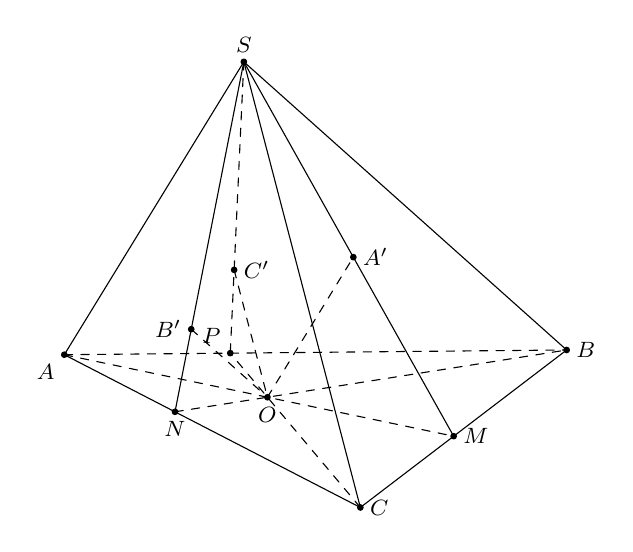
\begin{tikzpicture}[scale=1,font=\footnotesize,line join=round,line cap=round,>=stealth]
					 \draw (0.72,-1.76)-- (3.34,0.24);
					 \draw (-3.04,0.18)-- (0.72,-1.76);
					 \draw (-0.76,3.9)-- (-3.04,0.18);
					 \draw (-0.76,3.9)-- (0.72,-1.76);
					\draw  (-0.76,3.9)-- (3.34,0.24);
					\draw (1.905,-0.855)--  (-0.76,3.9);
					 \draw (-0.76,3.9)-- (-1.634,-0.545);
					\draw [dashed] (-3.04,0.18)-- (3.34,0.24); 
					\draw [dashed] (-3.04,0.18)--  (1.905,-0.855);
					\draw [dashed] (-0.46,-0.36)-- (0.631,1.419); 
					\draw [dashed]  (-0.76,3.9)-- (-0.932,0.2);
					\draw [dashed] (0.72,-1.76)--  (-0.932,0.2);
					\draw [dashed]  (-0.883,1.257)-- (-0.46,-0.36);
					\draw [dashed] (-1.634,-0.545)--  (3.34,0.24);
					 \draw [dashed] (-1.428,0.504)-- (-0.46,-0.36);
					\draw  [fill=] (-3.04,0.18) circle (1pt) node[below left] {$A$};
					\draw  [fill] (3.34,0.24) circle (1pt) node[right] {$B$};
					\draw  [fill] (0.72,-1.76) circle (1pt) node[right] {$C$};
					\draw  [fill] (-0.76,3.9) circle (1pt) node[above] {$S$};
					\draw [fill=] (-0.46,-0.36) circle (1pt)  node[below] {$O$};
					\draw [fill] (1.905,-0.855) circle (1pt) node[right] {$M$}; 
					 \draw [fill] (0.631,1.419) circle (1pt) node[right] {$A'$};
					 \draw [fill] (-0.932,0.2) circle (1pt) node[above left] {$P$};
					\draw [fill]  (-0.883,1.257) circle (1pt) node[right] {$C'$};
					\draw [fill] (-1.634,-0.545) circle (1pt) node[below] {$N$}; 
					\draw [fill] (-1.428,0.504) circle (1pt)  node[left] {$B'$};
				\end{tikzpicture}
		\end{center}
		Gọi $M$, $N$, $P$ lần lượt là giao điểm của $AO$ và $BC$, $BO$ và $AC$, $CO$ và $AB$.\\ 
		Ta có 
		\begin{itemize}
			\item 
			\begin{eqnarray*}
				 &\dfrac{OA'}{SA}&=\dfrac{MO}{MA}=\dfrac{S_{CMO}}{S_{CMA}}=\dfrac{S_{BMO}}{S_{BMA}}\\
				&&=\dfrac{S_{CMO}+S_{BMO}}{S_{CMA}+S_{BMA}}\\ 
				&&=\dfrac{S_{OBC}}{S_{ABC}}. 
			\end{eqnarray*}
			 \item
			\begin{eqnarray*}
				 &\dfrac{OB'}{SB}&=\dfrac{NO}{NB}=\dfrac{S_{ANO}}{S_{ANB}}=\dfrac{S_{CNO}}{S_{CNB}}\\
				 &&=\dfrac{S_{ANO}+S_{CNO}}{S_{ANB}+S_{CNB}}\\
				 &&=\dfrac{S_{OAC}}{S_{ABC}}.
			\end{eqnarray*}
			 \item
			\begin{eqnarray*}
				\dfrac{OC'}{SC}=\dfrac{PO}{PC}=\dfrac{S_{APO}}{S_{APC}} 
				=\dfrac{S_{BPO}}{S_{BPC}}=\dfrac{S_{APO}+S_{BPO}}{S_{APC}+S_{BPC}}=\dfrac{S_{OAB}}{S_{ABC}}. 
			\end{eqnarray*}
		\end{itemize}
		\noindent Từ  đó \[T=\dfrac{OA'}{SA}+\dfrac{OB'}{SB}+\dfrac{OC'}{SC}=\dfrac{S_{OBC}}{S_{ABC}}+\dfrac{S_{OAC}}{S_{ABC}}+\dfrac{S_{OAB}}{S_{ABC}}=\dfrac{S_{ABC}}{S_{ABC}}=1.\]
	} 
\end{ex}

% nguồn: Ok_TraLoiNgan_Lop11_Lan2
\begin{ex}%[1H4V2-4]%[ma:f3dcff99]
	Cho tứ diện $ABCD$. Gọi $ M$ là điểm thuộc cạnh $ BC$ sao cho $ MC=2MB$, các điểm $ N$, $ P$ lần lượt là trung điểm $ BD$, $ AD$ và $ Q$ là giao điểm của $ AC$ với  mặt phẳng $(MNP)$. Tỉ số $\dfrac{QA}{QC}$ bằng
	 \shortans{0,5}
	\loigiai{ 
		\begin{center}
			\begin{tikzpicture}[scale=1,line join=round,line cap=round,font=\footnotesize,>=stealth]
					\def\a{4} 
					\path (0:0) coordinate  (B)
						++(0:\a) coordinate (D) 
						 ++(-120:\a/2) coordinate (C)
						($(B)+(70:\a)$) coordinate (A) 
						($(B)!0.5!(D)$)  coordinate (N)
						($(A)!0.5!(D)$) coordinate  (P)
						($(B)!1/3!(C)$) coordinate (M) 
						 ($(A)!1/3!(C)$) coordinate (Q);
					 \draw[dashed,thick] (B)--(D)
						 (M)--(N)--(P);
					\draw[thick]  (P)--(Q)--(M)
						 (B)--(A)--(D)
						 (A)--(C)
						(B)--(C)--(D); 
					\foreach \x/\g  in {A/90,B/180,C/-45,D/0,N/-45,P/0,M/-170,Q/170}
					 \fill[black] (\x) circle (1pt)
						($(\g:3mm)+(\x)$) node {$\x$}; 
				\end{tikzpicture}
		\end{center}
		Vì $ NP$ là  đường trung bình của tam giác $ ABD$ nên $ NP \parallel AB$.\\
		 Ta có $\heva{&M\in\left(MNP\right)\cap\left(ABC\right)\\
		&NP \parallel AB\\ 
		&NP\subset\left(MNP\right)\\ 
		 &AB\subset\left(ABC\right).}$\\
		Nên giao tuyến của $\left(MNP\right)$ và $\left(ABC\right)$  là đường thẳng qua $ M$, song song với $ AB$.\\
		Qua  $ M$ kẻ đường thẳng song song với $ AB$, cắt $ AC$ tại $ Q$.\\
	Áp dụng định lý Ta-lét, ta có $\dfrac{QA}{QC}=\dfrac{MB}{MC}=\dfrac{1}{2} =  0{,}5$.}
\end{ex}

% nguồn: Ok_TraLoiNgan_Lop11_Lan2
\begin{ex}%[1H4V2-4]%[ma:61e082f8]
	Cho hình chóp $S.ABCD$ có đáy $ABCD$ là hình bình hành tâm $O$. Gọi $M$, $N$ lần lượt là trung điểm của $SC$, $OB$. Gọi $I$ là giao điểm của $SD$ và mặt phẳng $(AMN)$. Khi đó  tỉ số $\dfrac{SI}{DI}=\dfrac{a}{b}$ với $\dfrac{a}{b}$ là phân số tối giản và $a,b\in \mathbb{Z}$. Tính giá trị biểu thức $a+b$.
	 \shortans{5}
	\loigiai{ 
		\begin{center}
			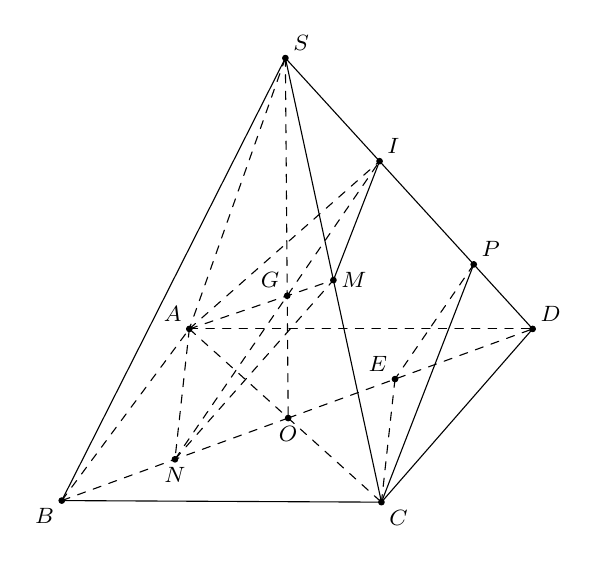
\begin{tikzpicture}[scale=1,font=\footnotesize,line join=round,line cap=round,>=stealth]
					\draw [dashed] (-2.06,0.86)--  (2.3,0.86);
					\draw  (2.3,0.86)-- (0.38,-1.34);
					\draw (0.38,-1.34)--  (-3.68,-1.32);
					\draw [dashed] (-3.68,-1.32)--  (-2.06,0.86);
					\draw [dashed] (-2.06,0.86)--  (0.38,-1.34);
					\draw  [dashed] (-0.84,4.3)-- (-2.06,0.86);
					\draw (-0.84,4.3)--  (-3.68,-1.32);
					\draw (-0.84,4.3)--  (0.38,-1.34);
					\draw (-0.84,4.3)--  (2.3,0.86);
					\draw [dashed] (-0.84,4.3)-- (-0.8047,-0.2718); 
					\draw [dashed] (-2.06,0.86)-- (-0.23,1.48); 
					\draw  [dashed] (-0.8047,-0.2718)-- (-3.68,-1.32);
					\draw  [dashed] (-0.8047,-0.2718)-- (2.3,0.86);
					\draw  [dashed] (-2.06,0.86)-- (-2.2424,-0.7959);
					\draw [dashed]  (-2.2424,-0.7959)-- (-0.23,1.48);
					\draw [dashed] (-2.2424,-0.7959)--  (0.356,2.99);
					\draw (-0.23,1.48)--  (0.356,2.99);
					 \draw [dashed] (1.5519,1.6795)-- (0.5521,0.2228);
					\draw (1.5519,1.6795)-- (0.38,-1.34); 
					\draw [dashed] (0.5521,0.2228)--  (0.38,-1.34);
					\draw [dashed]  (-2.06,0.86)-- (0.356,2.99);
					\begin{scriptsize}
						 \draw [fill] (-2.06,0.86) circle (1pt) node[above left] {$A$};
						 \draw [fill] (2.3,0.86) circle (1pt) node[above right] {$D$};
						 \draw [fill] (0.38,-1.34) circle (1pt) node[below right] {$C$};
						\draw [fill] (-3.68,-1.32) circle (1pt) node[below left] {$B$}; 
						\draw [fill] (-0.84,4.3)  circle (1pt) node[above right] {$S$};
						\draw [fill]  (-0.8047,-0.2718) circle (1pt) node[below] {$O$};
						\draw [fill] (-0.23,1.48) circle (1pt) node[right]  {$M$};
						 \draw [fill] (-0.8167,1.2812) circle (1pt) node[above left] {$G$};
						\draw [fill] (-2.2424,-0.7959) circle (1pt)  node[below] {$N$};
						\draw [fill] (0.356,2.99) circle (1pt) node[above right] {$I$}; 
						\draw [fill] (1.5519,1.6795) circle (1pt) node[above right]  {$P$};
						 \draw [fill] (0.5521,0.2228) circle (1pt) node[above left] {$E$};
					\end{scriptsize}
				\end{tikzpicture}
		\end{center}
		Trong $(SAC)$ gọi  $G=SO\cap AM$.\\
		Trong  $(SBD)$ gọi $I=NG\cap SD$ $\Rightarrow I=SD\cap (AMN)$.\\
		Trong $(SCD)$ kẻ $CP\parallel MI$.\qquad (1)\\ Do đó $MI$ là đường  trung bình của $\Delta SCP$ nên $ SI=IP$.\qquad (3)\\
		 Trong $(SBD)$ kẻ $PE\parallel NI$.\qquad (2)\\
		Từ $(1)$ và $(2)$ nên $(PEC)\parallel (ANMI)$.\\ 
		Mà $(ABCD)\cap (CPE)=CE$ và $(ABCD)\cap (ANMI)=AN$  nên $CE\parallel AN\Rightarrow \dfrac{OE}{ON}=\dfrac{OA}{OC}=1$.
		\noindent Ta có $OE=NO=\dfrac{1}{2}OB=\dfrac{1}{2}OD\Rightarrow E$ là trung điểm  của $OD$ và $DN=3DE$.\\
		Xét $\Delta NID$ có $PE\parallel NI\Rightarrow  \dfrac{DP}{DI}=\dfrac{DE}{DN}=\dfrac{1}{3}\Rightarrow DP=\dfrac{1}{3}DI\Rightarrow IP=\dfrac{2}{3}DI$.\qquad (4)\\
		Từ $(3)$ và $(4)\Rightarrow SI=\dfrac{2}{3}DI\Rightarrow \dfrac{SI}{DI}=\dfrac{2}{3}$ nên  $a=2;b=3$.\\
	Vậy $T=a+b=2+3=5$.} 
\end{ex}

% nguồn: Ok_TraLoiNgan_Lop11_Lan2
\begin{ex}%[1H4V2-4]%[ma:a57831bd]
	Cho hình chóp $S.ABCD$ có đáy $ABCD$ là hình bình hành. Gọi $A'$ là điểm trên $SA$ sao cho $A'A=\dfrac{1}{2}A'S$. Qua $A'$ kẻ đường thẳng song song với $AC$ cắt $SC$ tại $C'$. Mặt phẳng  $(\alpha)$ chứa $A'C'$ cắt các cạnh $SB$, $SD$ lần lượt tại $B'$, $D'$. Tính giá trị của biểu thức $T=\dfrac{SB}{SB'}+\dfrac{SD}{SD'}$.
	\shortans{3} 
	\loigiai{Gọi $O$ là  giao của $AC$ và $BD$ thì ta có $O$ là trung điểm của đoạn thẳng $AC$ và $BD$.\\
		 Các đoạn thẳng $SO$, $A'C'$, $B'D'$ đồng quy tại $I$.
	 \immini{
		Ta có 
		\begin{eqnarray*}
			&&S_{SA'I}+S_{SC'I}=S_{SA'C'}\\ 
			&\Leftrightarrow&\dfrac{S_{SA'I}}{S_{SAC}}+\dfrac{S_{SC'I}}{S_{SAC}}=\dfrac{S_{SA'C'}}{S_{SAC}}\\ 
			&\Leftrightarrow&\dfrac{S_{SA'I}}{2S_{SAO}}+\dfrac{S_{SC'I}}{2S_{SCO}}=\dfrac{S_{SA'C'}}{S_{SAC}}\\ 
			&\Leftrightarrow&\dfrac{SA'}{2SA}\cdot  \dfrac{SI}{SO}+\dfrac{SC'}{2SC}\cdot \dfrac{SI}{SO}=\dfrac{SA'}{SA}\cdot \dfrac{SC'}{SC}\\
			&\Leftrightarrow &\dfrac{SI}{2SO}\left(\dfrac{SA'}{SA}+\dfrac{SC'}{SC}\right)=\dfrac{SA'}{SA}.\dfrac{SC'}{SC}\\ 
			 &\Leftrightarrow&\dfrac{SA}{SA'}+\dfrac{SC}{SC'}=2\cdot \dfrac{SO}{SI}.
		\end{eqnarray*}
		 \noindent Tương tự $\dfrac{SB}{SB'}+\dfrac{SD}{SD'}=2\cdot \dfrac{SO}{SI}$.
		} 
		{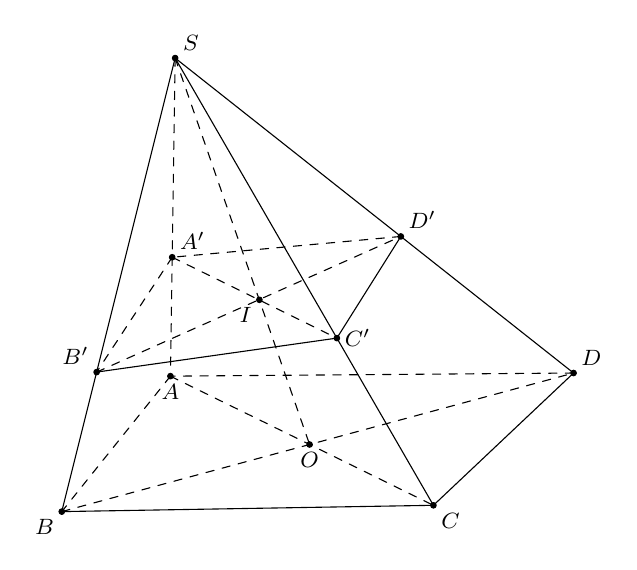
\begin{tikzpicture}[scale=1,font=\footnotesize,line join=round,line cap=round,>=stealth]
		\draw [dashed] (-1.4,0.82)-- (-2.78,-0.9); 
		\draw  (-2.78,-0.9)-- (1.94,-0.82);
		 \draw (1.94,-0.82)-- (3.72,0.86);
		 \draw [dashed] (3.72,0.86)-- (-1.4,0.82);
		 \draw [dashed] (-1.34,4.86)-- (-1.4,0.82);
		\draw  (-1.34,4.86)-- (-2.78,-0.9);
		\draw  (-1.34,4.86)-- (1.94,-0.82);
		\draw (-1.34,4.86)--  (3.72,0.86);
		\draw [dashed] (-1.4,0.82)-- (1.94,-0.82); 
		\draw [dashed] (-2.78,-0.9)-- (3.72,0.86); 
		\draw [dashed]  (-1.3776,2.3303)-- (-2.3371,0.8718);
		 \draw (-2.3371,0.8718)-- (0.7138,1.3033);
		\draw (0.7138,1.3033)--  (1.5261,2.5943);
		\draw [dashed] (1.5261,2.5943)-- (-1.3776,2.3303); 
		\draw [dashed]  (-1.3776,2.3303)-- (0.7138,1.3033);
		\draw [dashed] (-2.3371,0.8718)-- (1.5261,2.5943); 
		\draw [dashed]  (-1.34,4.86)-- (0.3673,-0.0478);
		\begin{scriptsize}
			\draw [fill] (-1.4,0.82) circle (1pt) node[below]  {$A$};
			 \draw [fill] (-2.78,-0.9) circle (1pt) node[below left] {$B$};
			\draw [fill] (1.94,-0.82) circle  (1pt) node[below right] {$C$};
			\draw [fill] (3.72,0.86) circle (1pt) node[above  right] {$D$};
			\draw [fill] (-1.34,4.86) circle (1pt)  node[above right] {$S$};
			\draw  [fill] (-1.3776,2.3303) circle (1pt) node[above right] {$A'$};
			\draw [fill] (-2.3371,0.8718) circle (1pt) node[above  left] {$B'$};
			\draw  [fill] (0.7138,1.3033) circle (1pt) node[right] {$C'$};
			\draw [fill] (1.5261,2.5943) circle (1pt) node[above right] {$D'$}; 
			\draw [fill] (0.3673,-0.0478) circle  (1pt) node[below] {$O$};
			\draw [fill]  (-.27,1.79) circle (1pt) node[below left] {$I$};
		\end{scriptsize}
	\end{tikzpicture}
		 }
		\noindent Ta có $A'C'\parallel AC$ nên $\dfrac{SA}{SA'}=\dfrac{SC}{SC'}=\dfrac{3}{2}$.\\ 
		 Do đó $\dfrac{SB}{SB'}+\dfrac{SD}{SD'}=\dfrac{SA}{SA'}+\dfrac{SC}{SC'}=\dfrac{3}{2}+\dfrac{3}{2}=3$.
	 }
\end{ex}

% nguồn: Ok_TraLoiNgan_Lop11_Lan2
\begin{ex}%[1H4V2-4]%[ma:59c2fac2]
	Cho tứ diện $ ABCD$. Các điểm $ P$, $Q$ lần lượt là trung điểm của $ AB$ và $ CD$; điểm $ R$ nằm trên cạnh $ BC$ sao cho $ BR=2RC$. Gọi $ S$ là giao điểm của $\left(PQR\right)$ và  cạnh $ AD$. Tính tỉ số $\dfrac{SA}{SD}$.
	 \shortans{2}
	\loigiai{ 
		\begin{center}
			\begin{tikzpicture}[scale=1,line join=round,line cap=round,font=\footnotesize,>=stealth]
					 \def\a{4}
					\path (0:0) coordinate (B) 
						++(0:\a) coordinate  (D)
						++(-120:\a/2) coordinate (C) 
						($(B)+(70:\a)$) coordinate  (A)
						 ($(A)!0.5!(B)$) coordinate (P)
						($(C)!0.5!(D)$) coordinate  (Q)
						($(B)!2/3!(C)$) coordinate  (R)
						($(A)!2/3!(D)$)  coordinate (S)
						(intersection  of P--S and R--Q) coordinate (I)
						($(R)!0.5!(I)$)  coordinate (E)
						($(P)!0.5!(I)$) coordinate  (F);
					\draw[dashed,thick]  (B)--(D)
						 (P)--(S)--(D)
						(R)--(Q) 
						 (F)--(D)--(I)
						(D)--(E) 
						(P)--(Q)--(D); 
					\draw[thick] (B)--(A)--(S) 
						 (A)--(C)
						(B)--(C) 
						 (S)--(I)--(Q)--(C)
						(P)--(R); 
					\foreach \x/\g in  {A/90,B/180,C/-45,D/45,P/170,Q/-80,R/-90,S/45,I/0,E/-90,F/45}
					 \fill[black] (\x) circle (1pt)
						 ($(\g:3mm)+(\x)$) node {$\x$};
				\end{tikzpicture}
		\end{center}
		Trong mặt phẳng  $\left(BCD\right)$, gọi $ I=RQ\cap BD$.\\
		 Trong $\left(ABD\right)$, gọi $S=PI\cap AD$ $\Rightarrow S=AD\cap\left(PQR\right)$.\\
		Trong mặt phẳng $\left(BCD\right)$, dựng $ DE \parallel BC$ $\Rightarrow DE$ là đường trung  bình của tam giác $ IBR$.\\
		$\Rightarrow D$ là trung điểm của $ BI$.\\ 
	Trong $\left(ABD\right)$, dựng $ DF \parallel AB$ $\Rightarrow \dfrac{DF}{BP}=\dfrac{1}{2} \Rightarrow  \dfrac{DF}{PA}=\dfrac{1}{2} \Rightarrow\dfrac{SA}{SD}=2$.}
\end{ex}

% nguồn: Ok_TraLoiNgan_Lop11_Lan2
\begin{ex}%[1H4V2-4]%[ma:c1a32591]
	Cho hình chóp $S.ABCD$ có đáy là hình bình hành. Gọi $M$,  $N$ lần lượt là trung điểm của $AB$, $AD$ và $G$ là trọng tâm của tam giác $SBD$. Mặt phẳng $(MNG)$ cắt $SC$ tại điểm $H$. Tính $\dfrac{SH}{SC}$.
	\shortans{0,4} 
	\loigiai{ 
		\begin{center}
			\begin{tabular}{p{8cm}p{8cm}}
				\begin{tikzpicture}[scale=1,line join=round,line cap=round,font=\footnotesize,>=stealth]
						 \def\a{4}
						\path (0:0)  coordinate (A)
						++(0:\a) coordinate (D) 
						 ++(-130:\a/2) coordinate (C)
						($(A)+(C)-(D)$)  coordinate (B)
						($(A)+(80:\a)$) coordinate (S) 
						($(A)!0.5!(B)$)  coordinate (M)
						($(A)!0.5!(D)$) coordinate  (N)
						(intersection of A--C and B--D)  coordinate (O)
						(intersection of A--C and  M--N) coordinate (E)
						 ($(S)!2/3!(O)$) coordinate (G)
						($(E)!3!(G)$) coordinate  (X)
						 (intersection of E--X and S--C) coordinate (H);
						\draw[dashed,thick] (B)--(A)--(D)--(B) 
						 (C)--(A)--(S)
						 (M)--(N)
						(S)--(O) 
						(E)--(G)--(H) 
						 (M)--(G)--(N);
						\draw[thick] (B)-- (C)--(D) 
						 (B)--(S)
						 (C)--(S)
						 (D)--(S);
						 \foreach \x/\g in {A/135,B/-135,C/-45,D/45,S/90,M/-30,N/60,O/-90,E/-90,G/140,H/20}
						\fill[black] (\x) circle (1pt) 
						($(\g:3mm)+(\x)$) node  {$\x$};
					\end{tikzpicture}
				 &
				\begin{tikzpicture}[scale=1,line join=round,line cap=round,font=\footnotesize,>=stealth]
						\def\a{5} 
						\path  (0:0) coordinate (A)
						++(0:\a)  coordinate (C)
						 ++(130:\a) coordinate (S)
						($(A)!0.5!(C)$)  coordinate (O)
						 ($(S)!2/3!(O)$) coordinate (G)
						($(A)!0.5!(O)$)  coordinate (E)
						 ($(E)!3!(G)$) coordinate (X)
						(intersection of  E--X and S--C) coordinate (H)
						($(S)!0.5!(H)$) coordinate (J) 
						 (intersection of A--J and S--O) coordinate (I);
						 \draw[thick] (A)--(S)--(C)--(A)
						(A)--(J) 
						 (E)--(H)
						(S)--(O); 
						\foreach \x/\g in {A/135,C/-45,S/90,O/-90,E/-90,G/140,H/20,I/20,J/20} 
						\fill[black]  (\x) circle (1pt)
						($(\g:3mm)+(\x)$) node {$\x$}; 
					\end{tikzpicture}
			\end{tabular}
		\end{center}
		 Trong mặt phẳng $(ABCD)$, gọi $E=MN\cap AC$.\\
		Trong mặt phẳng $(SAC)$, gọi  $H=EG\cap SC$.\\
		Ta có $\heva{&H\in EG \subset(MNG)\\&H\in SC}\Rightarrow H=SC \cap(MNG)$.\\ 
		Gọi $I$, $J$ lần lượt là trung  điểm của $SG$ và $SH$.\\
		Ta có $\heva{&IJ\parallel  HG\\&IA\parallel GE}\Rightarrow A,\,I,\,J$ thẳng hàng.\\
		Xét $\triangle ACJ$  có $EH\parallel AJ\Rightarrow \dfrac{CH}{HJ}=\dfrac{CE}{EA}=3\Rightarrow CH=3HJ$.\\
		Lại có  $SH=2HJ$ nên $SC=5HJ$.\\
		 Vậy $\dfrac{SH}{SC}=\dfrac{2}{5}$.
	} 
\end{ex}

% nguồn: Ok_TraLoiNgan_Lop11_Lan1
\begin{ex}%[1H4C2-4]%[ma:2b7dbddf]
	Cho hình chóp $S.ABC$. Bên trong tam giác $ABC$ ta lấy một điểm $O$ bất kỳ. Từ $O$ ta  dựng các đường thẳng lần lượt song song với $SA$, $SB$, $SC$ và cắt các mặt phẳng $\left( SBC \right)$, $\left( SCA \right)$, $\left( SAB \right)$ theo thứ tự tại $A'$, $B'$, $C'$. Khi đó tổng tỉ số $T=\dfrac{OA'}{SA}+\dfrac{OB'}{SB}+\dfrac{OC'}{SC}$ bằng bao nhiêu?
	\shortans{1} 
	\loigiai{ 
		\begin{center}
			\begin{tikzpicture}[line join=round,line cap=round,>=stealth,scale=1,font=\footnotesize]
					\foreach  \x/\y/\n in {0/0/A,4/-2/B,6/0/C} \coordinate (\n) at (\x,\y);
					\coordinate (S) at  ($(A)+(3,4)$);
					\coordinate (M) at ($(C)!1/2!(B)$); 
					\coordinate  (N) at ($(A)!1/2!(C)$);
					\coordinate (P) at ($(A)!1/2!(B)$); 
					\coordinate (O) at  ($(A)!2/3!(M)$);
					\coordinate (A')  at ($(S)!2/3!(M)$);
					\coordinate (B') at  ($(S)!2/3!(N)$);
					 \coordinate (C') at ($(S)!2/3!(P)$);
					\draw  (S)--(A)--(B)--(C)--(S)--(B)
						 (S)--(M)
						(S)--(P); 
					 \draw[dashed] (A)--(C)
						(S)--(N) 
						 (C)--(P)
						(A)--(M) 
						 (B)--(N)
						 (O)--(A')
						(O)--(B') 
						(O)--(C'); 
					\foreach \t/\g in  {S/90,A/180,B/-90,C/0,M/-60,N/125,P/-150,O/-110,A'/40,B'/180,C'/170}{
						\draw[fill=black] (\t) circle (1pt)  node[shift={(\g:8pt)}]{$ \t $};
					} 
				\end{tikzpicture}
		\end{center}
		Gọi $M$, $N$, $P$  lần lượt là giao điểm của $AO$ và $BC$, $BO$ và $AC$, $CO$ và $AB$.
		Ta  có
		\begin{itemize}
			\item  $\dfrac{OA'}{SA}=\dfrac{MO}{MA}=\dfrac{S_{CMO}}{S_{CMA}}=\dfrac{S_{BMO}}{S_{BMA}}=\dfrac{S_{CMO}+S_{BMO}}{S_{CMA}+S_{BMA}}=\dfrac{S_{OBC}}{S_{ABC}}$.
			\item $\dfrac{OB'}{SB}=\dfrac{NO}{NB}=\dfrac{S_{ANO}}{S_{ANB}}=\dfrac{S_{CNO}}{S_{CNB}}=\dfrac{S_{ANO}+S_{CNO}}{S_{ANB}+S_{CNB}}=\dfrac{S_{OAC}}{S_{ABC}}$. 
			\item $\dfrac{OC'}{SC}=\dfrac{PO}{PC}=\dfrac{S_{APO}}{S_{APC}}=\dfrac{S_{BPO}}{S_{BPC}}=\dfrac{S_{APO}+S_{BPO}}{S_{APC}+S_{BPC}}=\dfrac{S_{OAB}}{S_{ABC}}$. 
		\end{itemize}
		Từ  đó $T=\dfrac{OA'}{SA}+\dfrac{OB'}{SB}+\dfrac{OC'}{SC}=\dfrac{S_{OBC}}{S_{ABC}}+\dfrac{S_{OAC}}{S_{ABC}}+\dfrac{S_{OAB}}{S_{ABC}}=\dfrac{S_{ABC}}{S_{ABC}}=1$.
	 }
\end{ex}

% nguồn: Ok_TraLoiNgan_Lop11_Lan2
\begin{ex}%[1H4C2-4]%[ma:8ac02d0d]
	Cho hình chóp $S.ABCD$ có đáy $ABCD$ là hình bình hành. Gọi $G$ là trọng tâm tam giác $ABC$ và $M$ là trung điểm $SC$. Gọi $K$ là giao điểm của $SD$  với mặt phẳng $(AGM)$. Tính tỉ số $\dfrac{KS}{KD}$.
	 \shortans{0,5}
	 \loigiai{
		\begin{center}
			\begin{tikzpicture}[scale=1,line join=round,line cap=round,font=\footnotesize,>=stealth]
					 \def\a{4}
					\path (0:0)  coordinate (A)
						++(0:\a) coordinate (D) 
						++(-130:\a/2) coordinate (C) 
						 ($(A)+(C)-(D)$) coordinate (B)
						($(A)+(80:\a)$)  coordinate (S)
						(intersection  of A--C and B--D) coordinate (O)
						($(S)!0.5!(C)$)  coordinate (M)
						($(B)!2/3!(O)$)  coordinate (G)
						(intersection  of A--M and S--O) coordinate (I)
						 ($(G)!2!(I)$) coordinate (X)
						(intersection of G--X and S--D)  coordinate (K);
					\draw[dashed,thick] (B)--(A)--(D)--(B) 
						 (C)--(A)--(S)
						 (A)--(G)
						(G)--(K) 
						(A)--(M) 
						 (S)--(O)
						 (G)--(M);
					\draw[thick]  (B)-- (C)--(D)
						(B)--(S) 
						 (C)--(S)
						 (D)--(S);
					\foreach  \x/\g in {A/135,B/-135,C/-45,D/45,S/90,O/-90,M/0,G/-90,I/150,K/0}
					\fill[black] (\x) circle (1pt) 
						($(\g:3mm)+(\x)$) node  {$\x$};
				\end{tikzpicture}
		\end{center}
		 Gọi $O=AC\cap BD$, $I=AM\cap SO$.\\
		Trong mặt phẳng $(SBD)$, kéo dài $GI$ cắt $SD$ tại  $K\Rightarrow K=SD\cap(AMG)$.\\
		Trong tam giác $SAC$, có $SO$, $AM$ là hai đường  trung tuyến.\\
		Suy ra $I$ là trọng tâm tam giác  $SAC\Rightarrow\dfrac{OI}{OS}=\dfrac{1}{3}$.\\
		 Ta lại có $\dfrac{OG}{OB}=\dfrac{1}{3}\Rightarrow \dfrac{OI}{OS}=\dfrac{OG}{OB}\Rightarrow GI\parallel SB\Rightarrow GK\parallel SB\Rightarrow \dfrac{KD}{KS}=\dfrac{GD}{GB}$.\\
		Ta có $DO=BO=3GO\Rightarrow GD=4GO$,  $GB=2GO$.\\
		Vậy $\dfrac{KD}{KS}=\dfrac{GD}{GB}=\dfrac{4GO}{2GO}=2\Rightarrow \dfrac{KS}{KD}=\dfrac{1}{2}$. 
	 }
\end{ex}

% nguồn: Ok_TraLoiNgan_Lop11_Lan2
\begin{ex}%[1H4C2-4]%[ma:8fef2858]
	Cho hình chóp $S.ABC$. Bên trong tam giác $ABC$ ta lấy một điểm $O$ bất kỳ. Từ $O$ ta dựng các đường thẳng lần lượt song song với $SA$, $SB$, $SC$ và cắt các mặt phẳng $(SBC)$, $( SCA)$, $(SAB)$ theo thứ  tự tại $A'$, $B'$, $C'$. Khi đó tổng tỉ số $T=\dfrac{OA'}{SA}+\dfrac{OB'}{SB}+\dfrac{OC'}{SC}$ bằng bao nhiêu?
	\shortans{1} 
	\loigiai{ 
		\begin{center}
			\begin{tabular}{p{8cm}p{8cm}}
				\begin{tikzpicture}[scale=1,line join=round,line cap=round,font=\footnotesize,>=stealth]
						 \def\a{5}
						 \def\h{5}
						\path (0:0)  coordinate (A)
						++(0:\a) coordinate  (C)
						 ++(-150:4*\a/5) coordinate (B)
						($(B)!0.5!(C)$) coordinate (M) 
						 ($(A)!0.5!(B)$) coordinate (P)
						 ($(A)!0.5!(C)$) coordinate (N)
						(2,4) coordinate (S) 
						(intersection of A--M and P--C) coordinate (O) 
						($(S)!2/3!(M)$)  coordinate (A')
						 ($(S)!2/3!(P)$) coordinate (C')
						($(S)!2/3!(N)$) coordinate  (B');
						\draw[thick]  (A)--(B)
						 (B)--(C)
						(S)--(A) 
						 (S)--(B)
						(S)--(C) 
						 (S)--(M)
						(S)--(P); 
						\draw[dashed,thick] (A)--(C) 
						 (A)--(M)
						(C)--(P) 
						(S)--(N) 
						 (O)--(A')
						(O)--(B') 
						 (O)--(C');
						\foreach  \x / \goc in {B/-90,C/0,A/180,S/90,P/150,M/-45,O/-90,A'/0,B'/0,C'/180,N/150}
						\fill  (\x) circle (1.5pt)
						($(\x)+(\goc:3mm)$) node {$\x$}; 
					\end{tikzpicture}
				 &
				\begin{tikzpicture}[scale=1,line join=round,line cap=round,font=\footnotesize,>=stealth]
						 \def\a{5}
						\path  (0:0) coordinate (B)
						++(0:\a) coordinate (C) 
						++(130:\a)  coordinate (A)
						($(B)!1/3!(C)$)  coordinate (M)
						 ($(A)!2/3!(B)$) coordinate (P)
						(intersection of  A--M and C--P) coordinate (O)
						($(B)!3!(O)$) coordinate  (X)
						(intersection of A--C  and B--X) coordinate (N);
						\draw[thick]  (A)--(B)--(C)--(A)
						(A)--(M) 
						(B)--(N) 
						(C)--(P); 
						\foreach  \x/\g in {A/135,C/-45,B/135,O/-60,M/-90,N/0,P/180}
						\fill[black] (\x) circle  (1pt)
						($(\g:3mm)+(\x)$)  node {$\x$};
					\end{tikzpicture}
			\end{tabular}
		\end{center}
		Gọi  $M$, $N$, $P$ lần lượt là giao điểm của $AO$ và $BC$, $BO$ và $AC$, $CO$ và $AB$.\\
		Ta  có $$\dfrac{OA'}{SA}=\dfrac{MO}{MA}=\dfrac{S_{CMO}}{S_{CMA}}=\dfrac{S_{BMO}}{S_{BMA}}=\dfrac{S_{CMO}+S_{BMO}}{S_{CMA}+S_{BMA}}=\dfrac{S_{OBC}}{S_{ABC}};$$
		 $$\dfrac{OB'}{SB}=\dfrac{NO}{NB}=\dfrac{S_{ANO}}{S_{ANB}}=\dfrac{S_{CNO}}{S_{CNB}}=\dfrac{S_{ANO}+S_{CNO}}{S_{ANB}+S_{CNB}}=\dfrac{S_{OAC}}{S_{ABC}};$$
		$$\dfrac{OC'}{SC}=\dfrac{PO}{PC}=\dfrac{S_{APO}}{S_{APC}}=\dfrac{S_{BPO}}{S_{BPC}}=\dfrac{S_{APO}+S_{BPO}}{S_{APC}+S_{BPC}}=\dfrac{S_{OAB}}{S_{ABC}}.$$ 
		Từ đó  $$T=\dfrac{OA'}{SA}+\dfrac{OB'}{SB}+\dfrac{OC'}{SC}=\dfrac{S_{OBC}}{S_{ABC}}+\dfrac{S_{OAC}}{S_{ABC}}+\dfrac{S_{OAB}}{S_{ABC}}=\dfrac{S_{ABC}}{S_{ABC}}=1.$$
	 }
\end{ex}

% nguồn: Ok_TraLoiNgan_Lop11_Lan2
\begin{ex}%[1H4C2-4]%[ma:f8a3ac82]
	Cho tứ diện $ABCD$, $M$ là điểm thuộc $BC$ sao  cho $MC=3MB$. Gọi $N$, $P$ lần lượt là trung điểm của $BD$ và $AD$. Điểm $Q$ là giao điểm của $AC$ với $(MNP)$. Tính $\dfrac{QC}{QA}$.
	 \shortans{3}
	\loigiai{ 
		\begin{center}
			\begin{tikzpicture}[scale=1,line join=round,line cap=round,font=\footnotesize,>=stealth]
					\def\a{5} 
					\def\h{4} 
					\path  (0:0) coordinate (A)
						++(0:\a)  coordinate (C)
						++(-150:4*\a/5)  coordinate (B)
						($(A)!0.5!(B)$) coordinate (X) 
						 ($(C)!2/3!(X)$) coordinate (H)
						($(H)+(90:\h)$) coordinate (D) 
						($(A)!0.5!(D)$) coordinate (P) 
						($(D)!0.5!(B)$)  coordinate (N)
						($(C)!3/4!(B)$) coordinate (M) 
						($(C)!3/4!(A)$) coordinate  (Q);
					 \draw[thick] (C)--(B)
						(C)--(D) 
						(B)--(A) 
						(D)--(A) 
						(C)--(A) 
						(P)--(N)--(M); 
					\draw[dashed,thick]  (B)--(D)
						 (M)--(Q)--(P);
					\foreach \x / \goc in {B/-90,D/90,C/0,A/180,P/120,Q/-100,M/-30,N/0} 
					 \fill (\x) circle (1.5pt)
						($(\x)+(\goc:3mm)$) node  {$\x$};
				\end{tikzpicture}
		\end{center}
		Ta  có $\heva{&NP\parallel AB\\&NP\subset (MNP)\\&AB\subset(ABC)\\&M\in(ABC)\cap(MNP)}$.\\
		Do đó giao tuyến của $(ABC)$ và $(MNP)$ là đường thẳng $MQ\parallel  AB\,(Q\in AC)$.\\
		 Ta có $\dfrac{QC}{QA}=\dfrac{MC}{MB}=3$.\\
		Vậy $\dfrac{QC}{QA}=3$. 
	 }
\end{ex}

% nguồn: Ok_TraLoiNgan_Lop11_Lan2
\begin{ex}%[1H4C2-4]%[ma:3bfcf91d]
	Cho hình chóp $S.ABCD$ có đáy là hình thang ($AB\parallel CD$ và $AB=3CD$). Gọi $H$ là điểm thuộc cạnh $SC$  sao cho $SH=3HC$. Gọi $K$ là giao điểm của $SB$ và $(ADH)$. Tính tỉ số $\dfrac{SK}{SB}$.
	\shortans{0,5} 
	 \loigiai{
		\begin{center}
			\begin{tikzpicture}[scale=1,line join=round,line cap=round,font=\footnotesize,>=stealth]
					\def\a{5} 
					\path (0:0) coordinate (A) 
						++(0:\a) coordinate  (B)
						 ++(-130:\a/2) coordinate (C)
						($(A)+(C)-(B)$) coordinate (X) 
						($(C)!1/3!(X)$) coordinate (D) 
						 ($(A)+(80:3*\a/4)$) coordinate (S)
						($(S)!3/4!(C)$) coordinate  (H)
						(intersection of A--D  and B--C) coordinate (I)
						 ($(I)!3!(H)$) coordinate (Y)
						(intersection of I--Y  and S--B) coordinate (K)
						($(S)!4/3!(K)$)  coordinate (N);
					\draw[dashed,thick]  (A)--(B)
						(A)--(H) 
						 (C)--(D);
					\draw[thick]  (S)--(A)--(D)--(C)--(B)--(S)
						(S)--(D) 
						(S)--(C) 
						(I)--(K) 
						 (C)--(N)
						(I)--(D)--(H) 
						 (I)--(C);
					\foreach \x/\g  in {A/180,B/0,C/-90,D/-90,S/90,H/-20,I/-90,K/20,N/20}
					\fill[black] (\x) circle  (1pt)
						($(\g:3mm)+(\x)$)  node {$\x$};
				\end{tikzpicture}
		\end{center}
		\begin{itemize}
			\item  Xác định giao điểm $K$ của $SB$ và mặt phẳng $(ADH)$.\\
			Trong mặt  phẳng $(ABCD)$ gọi $I=AD\cap BC\Rightarrow \heva{&I\in AD\\&I\in BC.}$\\
			Xét hai mặt phẳng  $(ADH)$ và $(SBC)$ có\\
			$\heva{&I\in AD\subset  (ADH)\\&I\in BC\subset(SBC)}\Rightarrow I$ là điểm chung thứ nhất.\\
			$\heva{&H\in  (ADH)\\&H\in SC\subset(SBC)}\Rightarrow H$ là điểm chung thứ hai.\\
			Vậy  $(ADH)\cap(SBC)=IH$.\\
			Trong mặt phẳng $(SBC)$, gọi $K=IH\cap SB\Rightarrow  \heva{&K\in IH\subset(AIH)\\&K\in SB.}$\\
			Vậy $K=SB\cap(AHD)$. 
			\item Tính tỉ số $\dfrac{SK}{SB}$.\\ 
			 Từ $C$ dựng đường thẳng song song với $IK$, cắt $SB$ tại $N$.\\
			Xét $\triangle  SNC$ ta có $\dfrac{SK}{KN}=\dfrac{SH}{HC}=3$.\\
			Xét $\triangle KBI$ ta có $\dfrac{BK}{KN}=\dfrac{BI}{IC}$.\\ 
			Xét  $\triangle IAB$ ta có $\dfrac{IB}{IC}=\dfrac{AB}{DC}=3$.\\
			Suy ra  $\dfrac{SK}{KN}=\dfrac{BK}{KN}=3\Rightarrow SK=BK$.\\
			Vậy  $\dfrac{SK}{SB}=\dfrac{1}{2}$.
		\end{itemize}
	} 
\end{ex}

% nguồn: Ok_TraLoiNgan_Lop11_Lan2
\begin{ex}%[1H4C2-4]%[ma:4ad1eb1f]
	Cho hình chóp tứ giác đều $S.ABCD$ có cạnh đáy bằng  $10$. $M$ là điểm trên $SA$ sao cho $\dfrac{SM}{SA}=\dfrac{2}{3}$. Một mặt phẳng $(\alpha)$ đi qua $M$ song song với $AB$ và $BC$, cắt hình chóp theo một tứ giác có diện tích là
	 \shortans{44,4}
	\loigiai{ 
		\begin{center}
			\begin{tikzpicture}[scale=1,line join=round,line cap=round,font=\footnotesize,>=stealth]
					\def\a{4} 
					\path (0:0) coordinate  (A)
						++(0:\a)  coordinate (D)
						++(-130:\a/2) coordinate  (C)
						($(A)+(C)-(D)$) coordinate (B) 
						(intersection of A--C and  B--D) coordinate (O)
						($(O)+(90:1.25*\a)$) coordinate  (S)
						($(S)!2/3!(A)$) coordinate (M) 
						 ($(S)!2/3!(B)$) coordinate (N)
						 ($(S)!2/3!(C)$) coordinate (P)
						($(S)!2/3!(D)$)  coordinate (Q);
					 \draw[dashed,thick] (B)--(A)--(D)
						(A)--(S) 
						 (N)--(M)--(Q);
					\draw[thick] (B)--  (C)--(D)
						 (B)--(S)
						 (C)--(S)
						 (D)--(S)
						(N)--(P)--(Q); 
					\foreach  \x/\g in {A/-90,B/-135,C/-45,D/45,S/90,M/40,N/180,P/0,Q/0}
					\fill[black] (\x) circle  (1pt)
						($(\g:3mm)+(\x)$) node {$\x$}; 
					\fill[pattern=north west lines]  (M)--(N)--(P)--(Q)--(M);
				\end{tikzpicture}
		\end{center}
		Mặt phẳng $(\alpha)$ đi qua $M$ và song song với $AB$ nên từ $M$ kẻ đường thẳng song song với $AB$ cắt $SB$ tại $N$, từ $N$ kẻ đường thẳng song song với $BC$ cắt $SC$ tại $P$. Từ $P$ kẻ đường thẳng song song với $CD$ cắt $SD$ tại $Q$. Khi đó mặt phẳng $(\alpha)$ cắt hình chóp theo tứ giác $MNPQ$.\\ 
		Ta có tứ giác $MNPQ$ là hình vuông  có cạnh $MN=\dfrac{2}{3}\cdot AB=\dfrac{20}{3}$.\\
		Vậy diện tích tứ  giác $MNPQ$ là $S=\left(\dfrac{20}{3}\right)^2=\dfrac{400}{9}\approx 44,4$.
	 }
\end{ex}

% nguồn: Ok_TraLoiNgan_Lop11_Lan2
\begin{ex}%[1H4C2-4]%[ma:23af510c]
	Cho hình chóp $S.\,ABCD$ có đáy là hình  bình hành. Gọi $N$ là trung điểm của cạnh $SC$. Lấy điểm $M$ đối xứng với $B$ qua $A$. Gọi giao điểm $G$ của đường thẳng $MN$ với mặt phẳng $\left( SAD \right)$. Tính tỉ số $\frac{GM}{GN}$.
	 \shortans{2}
	\loigiai{ 
		\begin{center}
			\begin{tikzpicture}[scale=1,line join=round,line cap=round,font=\footnotesize,>=stealth]
					 \def\a{4}
					\path (0:0) coordinate  (A)
						++(0:\a) coordinate  (B)
						++(-80:\a/2)  coordinate (C)
						($(A)+(C)-(B)$) coordinate (D) 
						($(A)+(70:\a)$) coordinate  (S)
						(intersection of A--C and  B--D) coordinate (O)
						 ($(S)!0.5!(C)$) coordinate (N)
						($(B)!2!(A)$) coordinate  (M)
						($(A)!0.5!(B)$) coordinate (I) 
						(intersection of M--O and A--D) coordinate  (K)
						($(M)!2/3!(N)$) coordinate (G); 
					\draw[dashed,thick]  (M)--(B)
						(M)--(O) 
						 (A)--(C)
						 (B)--(D)
						(A)--(D) 
						(G)--(K) 
						 (O)--(N)
						 (G)--(N)
						(O)--(I); 
					\draw[thick]  (S)--(A)
						(S)--(B)--(C)--(D)--(S) 
						 (S)--(C)
						 (S)--(D)
						(M)--(G) 
						(M)--(D); 
					\foreach \x/\g in {A/135,B/0,C/-90,D/-90,S/90,O/-90,M/180,N/0,G/90,K/-150,I/90} 
					\fill[black] (\x)  circle (1pt)
						($(\g:3mm)+(\x)$)  node {$\x$};
				\end{tikzpicture}
		\end{center}
		Gọi giao điểm của $AC$ và $BD$ là $O$ và kẻ $OM$ cắt $AD$ tại $K$.\\ 
		Vì $O$ là trung điểm ${AC}$, $N$  là trung điểm ${SC}$ nên $ON\parallel SA$.\\
		Vậy hai mặt phẳng $(MON)$ và $(SAD)$ cắt nhau tại giao tuyến ${GK}$ song  song với ${NO}$.\\
		Áp dụng định lí Thalet  cho $\triangle MON$ có $GK\parallel ON$, ta có $\dfrac{GM}{GN}=\dfrac{KM}{KO}$.\\
		Gọi $I$ là trung điểm của ${AB}$, vì $O$ là trung điểm của ${BD}$ nên theo  tính chất đường trung bình ta suy ra $OI\parallel AD$.\\
		 Vậy theo định lí Thalet ta có $\dfrac{KM}{KO}=\dfrac{AM}{AI}=\dfrac{AB}{AI}=2$.\\
		 Do đó $\dfrac{GM}{GN}=2$.
	} 
\end{ex}
